\chapter{Resultados y discusión}

Uno de los objetivos principales de esta tesis fue desarrollar un programa de cómputo científico para explorar la posible aplicación del análisis multifractal en estructuras proteicas, por lo tanto, el programa podría ser una herramienta útil para caracterizar las distintas etapas del plegamiento proteico, describiéndolas en términos de la dinámica de formación de agregados estructurales, lo que permitiría una comprensión más profunda de estos procesos. Para mejorar la compresión de este trabajo, se ha dividido la descripción del programa \textit{\textbf{molmassfractraldim}} en dos secciones; el algoritmo y su uso para la obtención de resultados. 
 
 
\section{Algoritmo (diseño del programa)}

El propósito principal del programa \textbf{\textit{molmassfractaldim}} es determinar la dimesi\'{o}n fractal de masa mediante la caracterizaci\'{o}n de la geometría interna de un sistema proteico. Esto se logra construyendo una tabla de $r_{k}$, $\langle N(r_k) \rangle$, $\langle M(r_k) \rangle$ y $\langle Rg(r_k) \rangle$: donde;

\begin{itemize}
	\item $r_{k}$ es el radio de medida centrado en posiciones aleatorias de una prote\'{i}na con valores m\'{i}nimos y m\'{a}ximos definidos como $r_{min}$ y $r_{max}$.
	\item $\langle N(r_k) \rangle$ es el número promedio de partículas contenidas dentro de un radio $r_{k}$. 
	\item  $\langle M(r_k) \rangle$ es el n\'{u}mero de masa promedio de las part\'{i}culas contenidas en el radio $r_{k}$.
	\item  $\langle Rg(r_k) \rangle$ es el radio de giro promedio de las part\'{i}culas contenidas en el radio $r_{k}$.
\end{itemize}

Posteriormente, los valores de $\langle N(r_k) \rangle$, $\langle M(r_k) \rangle$ y $\langle Rg(r_k) \rangle$ pueden analizarse mediante regresiones lineales para determinar la dimensi\'{o}n fractal de masa. El procedimiento general del programa \textbf{\textit{molmassfractaldim}} se describe en el diagrama de flujo de la figura \ref{dfMolFractalDim}, cuyos pasos se explican en las siguientes subsecciones.
 
 
 \begin{figure}[h!]
 	\begin{center}
 		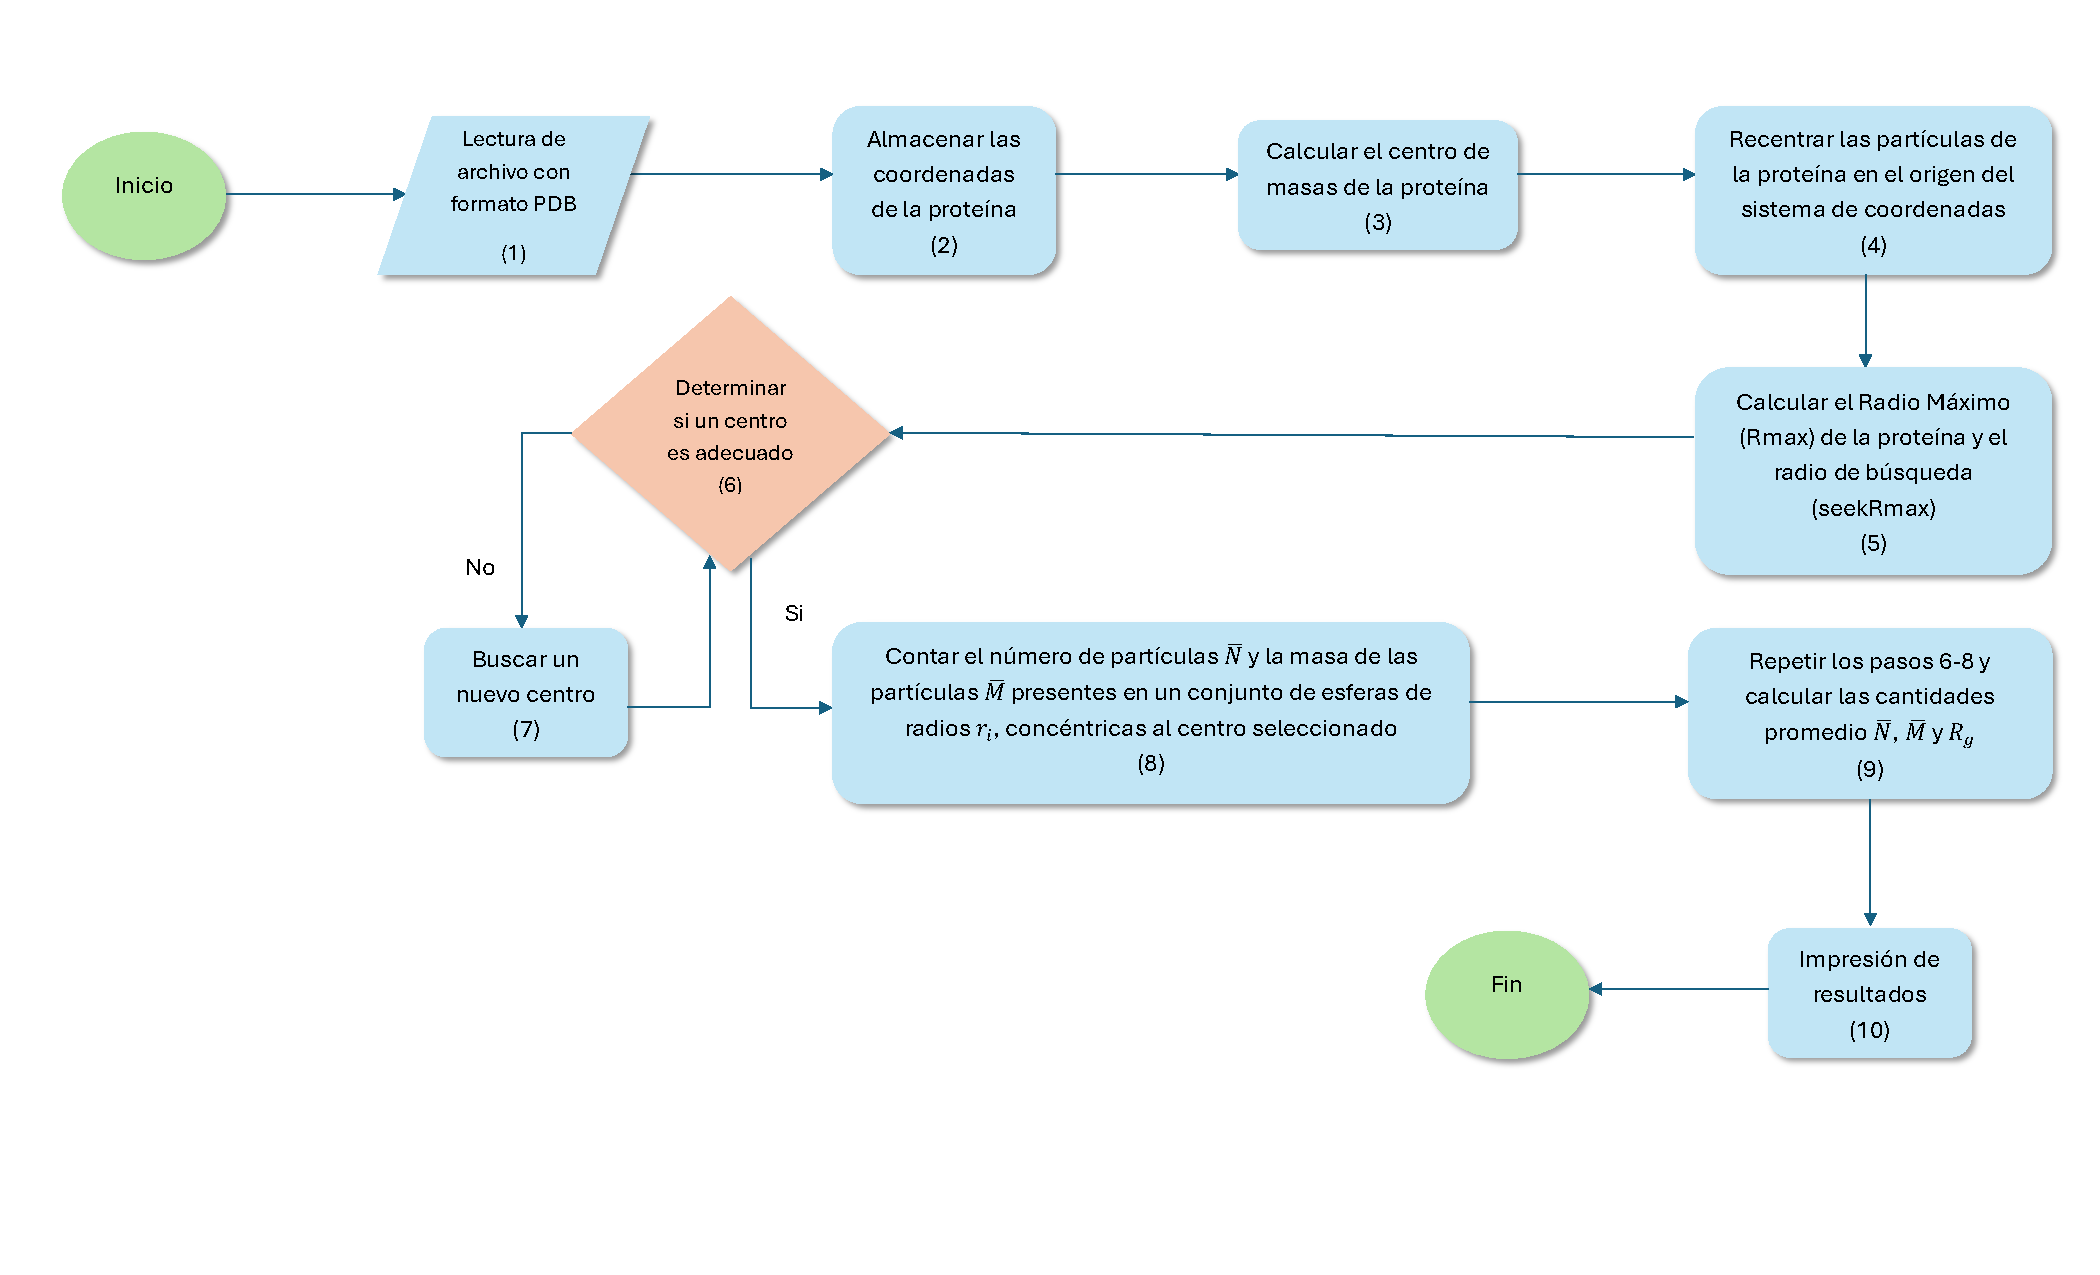
\includegraphics[width=\textwidth]{graphs/dfMolFractalDim}
 		\caption{Diagrama de flujo general del programa \textit{molmassfractaldim}.}
 		\label{dfMolFractalDim}
 	\end{center}
 \end{figure}
 
  	\color{blue}
 \subsection {Pasos 1, 2, 3 y 4 del diagrama de flujo general}
 
	\begin{itemize}
		\item \textbf{Paso 1:}
		Sea $\mathcal{M}$ un sistema molecular compuesto por un conjunto de partículas $N_{\text{at}}$. Cada partícula $i$ está descrita por la terna 
		
		\begin{equation}
			\mathcal{M} (\mathbf{r}_i, m_i, Z_i)
		\end{equation}
		
		donde $\mathbf{r}_i$ es el vector de posición, $m_i$ la masa y $Z_i$ el número atómico. El sistema completo se representa como	
		
		\begin{equation}
			\mathcal{M} = \bigl\{(\mathbf{r}_i, m_i, Z_i) \,\big|\, i = 1,\dots,N_{\text{at}}\bigr\}
		\end{equation}
	
		\item \textbf{Paso 2}: Para usar las posiciones de las partículas $i$ de $\mathcal{M}$ se define una matriz $\mathbf{X}$, que servirá como base para todos los cálculos posteriores:
		\begin{equation}
			\mathbf{X} = \begin{bmatrix}
				x_1 & y_1 & z_1 \\
				x_2 & y_2 & z_2 \\
				\vdots & \vdots & \vdots \\
				x_{N_{\text{at}}} & y_{N_{\text{at}}} & z_{N_{\text{at}}}
			\end{bmatrix} \in \mathbb{R}^{N_{\text{at}} \times 3}
		\end{equation}
		
		Donde la $i$-ésima fila es la traspuesta $\mathbf{r}_i^{\mathsf T}$.
		
		
		\item \textbf{Paso 3}: El centro de masas $\mathbf{r}_{\text{cm}}$ del sistema $\mathcal{M}$ se calcula como:
		\begin{equation}
			\mathbf{r}_{\text{cm}}
			= \frac{\displaystyle \sum_{i=1}^{N_{\text{at}}} m_i \mathbf{r}_i}
			{\displaystyle \sum_{i=1}^{N_{\text{at}}} m_i}
			\in \mathbb{R}^3
		\end{equation}
		que representa el punto de equilibrio mecánico del sistema $\mathcal{M}$. 
		Donde $\displaystyle \sum_{i=1}^{N_{\text{at}}} m_i \mathbf{r}_i$ es la suma de la posiciones ponderadas por las masas y $\displaystyle \sum_{i=1}^{N_{\text{at}}} m_i$ es la masa total del sistema.
		
		
		\item \textbf{Paso 4}: Se trasladan las coordenadas de $\mathcal{M}$ a su centro de masa:
		\begin{equation}
			\mathbf{r}_i' = \mathbf{r}_i - \mathbf{r}_{\text{cm}}, \qquad
			i=1,\dots,N_{\text{at}}
		\end{equation}
		
		Esto garantiza que
		\begin{equation}
			\sum_{i=1}^{N_{\text{at}}} m_i \mathbf{r}_i' = \mathbf{0}
		\end{equation} 
		
		donde $\mathbf{r}_i'$ es la posición de la partícula $i$ medida 
		con respecto al centro de masa del sistema $\mathcal{M}$. 
		$r_cm$ es el vector del centro de masa del sistema $\mathcal{M}$.
		
		
	\end{itemize}


	\subsection{Paso 5 del diagrama de flujo general}
	
	\begin{itemize}
		
		\item \textbf{Radio máximo}. Se define el radio máximo del sistema $\mathcal{M}$, calculado como la distancia máxima desde el origen hasta la partícula más lejana del sistema.
		
		\begin{equation}
			R_{\text{max}} = \max_i \|\mathbf{r}_i'\|
		\end{equation}
		
		
		
		\item \textbf{Radio de búsqueda}. Se define un radio que asegure que los puntos de medición no se encuentren cerca de los límites del sistema, con un valor del 75\% tamaño de $\mathcal{M}$, donde $\alpha = 0.75$.
		\begin{equation}
			R_{\text{seek}} = \alpha \cdot R_{\text{max}}
		\end{equation}
		
		
		\item \textbf{Radio de medición}. Se define  un conjunto de radios de medición como $nr$ con un incremento radial $dr$:
		\begin{equation}
			nr = 50 
		\end{equation}
		
		\begin{equation}
			dr = \frac{r_{max}-r_{min}}{nr-1}
		\end{equation}
		
		donde 
		
		\begin{equation}
			r_{min} = 0.15\, R_{\text{max}}, \qquad
			r_{max} = 20
		\end{equation}
		
		
		\item \textbf{Radio de medición local.} Para cada centro de muestreo se define
		un centro local
		\begin{equation}
			r_{loc} = \beta R_{\text{max}}, \qquad \beta = 0.15
		\end{equation} 
		
		donde $\beta$ limita el tamaño de las esferas a $15\%$ de $R_{max}$.
		
		\item \textbf{Centros de medición válidos.} 
		Un centro $\mathbf{r}_c$ puede usarse como centro sólo si
		
		\begin{equation}
			\|\mathbf{r}_c\| + r_{\mathrm{loc}} \le R_{\text{seek}}
		\end{equation}
		Esta condición asegura que la esfera de radio $r_{\text{loc}}$ quede completamente dentro de la región de muestreo.
		\end{itemize}

	 
	 
	 \subsection{Paso 6 y 7 del diagrama de flujo general}
	 
	 En este paso se utiliza un criterio llamado densidad de particulas promedio \(\rho_{P}\) que tiene como objetivo determinar cuando un centro local (ver paso 6 del diagrama de flujo presentado en la Fig. \ref{dfMolFractalDim}) no es adecuado para realizar la medici\'{o}n de la dimensi\'{o}n fractal. Por ejemplo, si una esfera de cierto radio centrada en alg\'{u}n punto de la proteína tiene una $\rho < 0.034$, ser\'{i}a altamente probable que la esfera intersecte en una zona considerada como un hueco de la prote\'{i}na. Un centro con tales caracter\'{i}sticas podr\'{i}a ser descartado hasta que se encuentre otro centro adecuado (ver bucle 6 $\longleftrightarrow$ 7 en la Figura \ref{dfMolFractalDim}). Visualmente este criterio se observa en la Figura \ref{fig:centrob}. 
	 
	 	\begin{figure}[H]
	 	\centering
	 	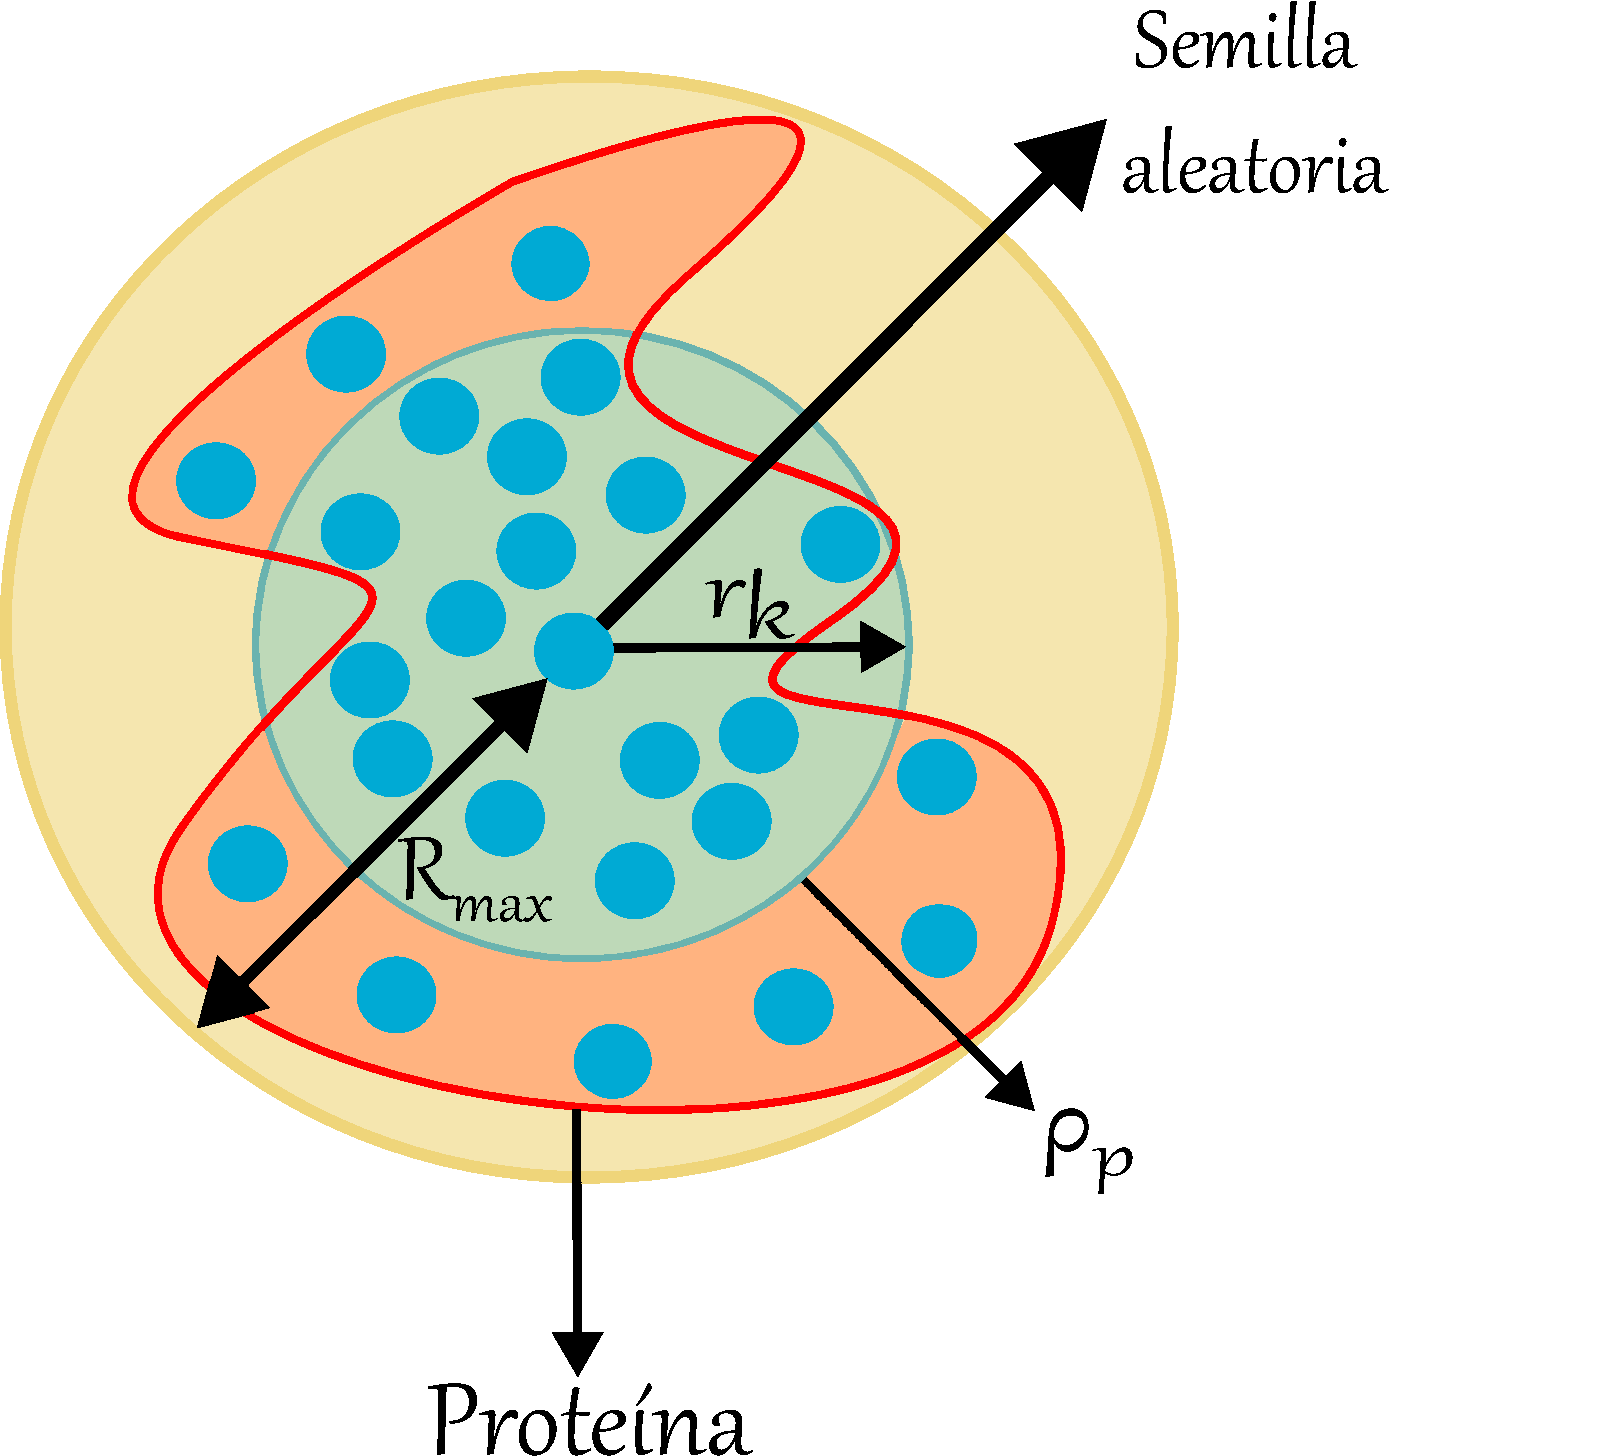
\includegraphics[width=0.5\linewidth]{graphs/centrob4.pdf}
	 	\caption{Diagrama 2D del c\'{a}lculo de la dimensi\'{o}n fractal de masa en prote\'{i}nas mediante \textit{molfractaldim}. (1) Se define un radio m\'{a}ximo en la prote\'{i}na ($R_{max}$) alrededor del centro de masa del sistema, (2) se determina si un centro local es adecuado ($\rho_{p} \geq 0.34$). Estas cantidades se utilizan para calcular la masa promedio de las part\'{i}culas $\bar{M}(r_k)$.}
	 	\label{fig:centrob}
	 \end{figure}
	 
	  Además de lo anterior, el criterio de \(\rho_{P}\) permite refinar la medici\'{o}n de $\langle N(r_k) \rangle$, $\langle M(r_k) \rangle$ y $\langle Rg(r_k) \rangle$, que a su vez son las relaciones que se utilizan para medir dimensiones fractales y as\'{i}, determinar si existe o no multifractalidad en estructuras proteicas. Este criterio calcula dos valores clave: (1) el volumen de cada esfera de radio \(r_k\) y (2) la densidad de partículas promedio presente en cada esfera de radio \(r_i\). El volumen de cada esfera se calcula usando el radio \(r_k\) de las esferas definidas anteriormente y a partir de la ecuaci\'{o}n \ref{volumen}.\\
	 
	 
	 \begin{equation}
	 	V(r_k) = \frac{4}{3} \pi r_{k}^{3}
	 	\label{volumen}
	 \end{equation}
	 
	 La densidad de part\'{i}culas promedio se calcula a partir de la ecuaci\'{o}n \ref{eq:densidad}. \\
	 Donde \(\rho_{P}\) es la densidad de part\'{i}culas promedio presentes en una esfera de radio \(r_k\).\\
	 \(\bar N(r_{k})\) es la cantidad promedio de part\'{i}culas presentes en una esfera de radio \(r_k\).
	 \(V_{k}\) es el volumen de una esfera de radio \(r_{k}\).
	 
	 \begin{equation}
	 	\rho_P = \frac{\bar N(r_{k})}{V_{k}}
	 	\label{eq:densidad}
	 \end{equation}
	 

	\subsection{Paso 8 del diagrama de flujo general}

	Para cada radio $r_k$ en la malla $\{r_{\text{min}}, r_{\text{min}} + \Delta r, \ldots, r_{\text{max}}\}$, se definen:
	
	\begin{equation}
		N(\mathbf{r}_c, r_k) = \sum_{i=1}^{N_{\text{at}}} 
		\Theta\!\bigl(r_k - \|\mathbf{r}_i' - \mathbf{r}_c\|\bigr)
	\end{equation}
	
	\begin{equation}
		M(\mathbf{r}_c, r_k) = \sum_{i=1}^{N_{\text{at}}} 
		m_i \cdot \Theta\!\bigl(r_k - \|\mathbf{r}_i' - \mathbf{r}_c\|\bigr)
	\end{equation}
	
	\begin{equation}
		R_g(\mathbf{r}_c, r_k) = 
		\sqrt{\frac{\displaystyle\sum_{i=1}^{N_{\text{at}}} 
				\|\mathbf{r}_i' - \mathbf{r}_c\|^2 \cdot 
				\Theta\!\bigl(r_k - \|\mathbf{r}_i' - \mathbf{r}_c\|\bigr)}
			{N(\mathbf{r}_c, r_k)}}.
	\end{equation}
	
	donde
	\begin{itemize}
		\item $\mathbf{r}_c$ es el centro de muestreo dentro del sistema.
		\item $\mathbf{r}_i'$ es la posición del partícula $i$ respecto al centro de masa.
		\item $m_i$ es la masa del partícula $i$.
		\item $\Theta(x)$ es la función de Heaviside que permite contar sólo los átomos dentro de la esfera, igual a $1$ si $x \ge 0$ y $0$ si $x < 0$. 
		\item $N(\mathbf{r}_c, r_k)$ es número de partículas dentro de la esfera de radio $r_k$.
		\item $M(\mathbf{r}_c, r_k)$ es masa total dentro de esa esfera.
		\item $R_g(\mathbf{r}_c, r_k)$ es radio de giro de las partículas en la esfera.
	\end{itemize}
	
	\textbf{Cálculo de valores promedio sobre múltiples centros}. Se seleccionan aleatoriamente centros de muestreo en $\{\mathbf{r}_{c_j}\}$:
	
	
	\begin{equation}
		N_{\text{meas}} = 30  
	\end{equation}
	
	Para calcular el valor de $\langle N(r_k) \rangle$, $\langle M(r_k) \rangle$ y $\langle Rg(r_k) \rangle$:
	
	\begin{equation}
		\langle N(r_k) \rangle = \frac{1}{N_{\text{meas}}} 
		\sum_{j=1}^{N_{\text{meas}}} N(\mathbf{r}_{c_j}, r_k)
	\end{equation}
	
	\begin{equation}
		\langle M(r_k) \rangle = \frac{1}{N_{\text{meas}}} 
		\sum_{j=1}^{N_{\text{meas}}} M(\mathbf{r}_{c_j}, r_k)
	\end{equation}
	
	\begin{equation}
		\langle R_g(r_k) \rangle = \frac{1}{N_{\text{meas}}} 
		\sum_{j=1}^{N_{\text{meas}}} R_g(\mathbf{r}_{c_j}, r_k).
	\end{equation}
	
	Donde:
	\begin{itemize}
		\item $N_{\text{meas}}$ es el número de centros aleatorios sobre los que se promedia.
		\item $\mathbf{r}_{c_j}$ es el vector de posición del j-ésimo centro de medición.
		\item $\langle\cdot\rangle$ es el promedio estadístico sobre todos los centros.
	\end{itemize}

		\begin{figure}[H]
		\subsection*{ Número de medidas -a A = 1 y 200}	
		\hspace{-0.3cm} 
		\begin{minipage}{0.49\textwidth}
			\centering
			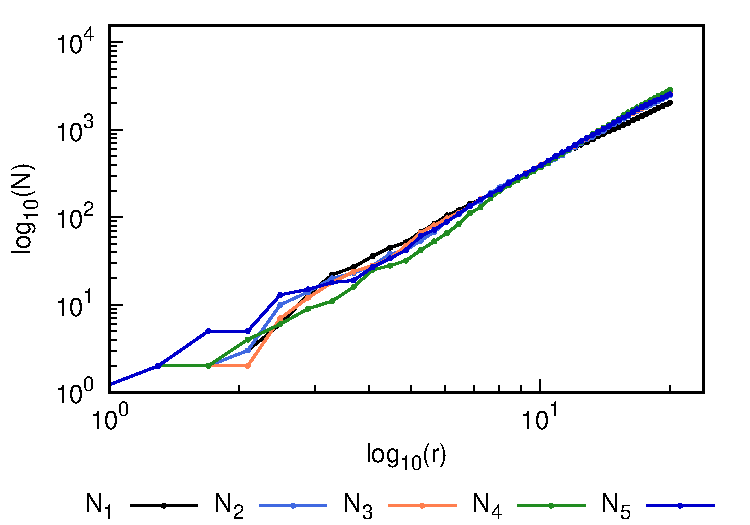
\includegraphics[width=\linewidth,page=1]{graphs/PDBs/Tubb4/TubMutA=1.pdf}
		\end{minipage}
		\hspace{0.2cm}
		\begin{minipage}{0.49\textwidth}
			\centering
			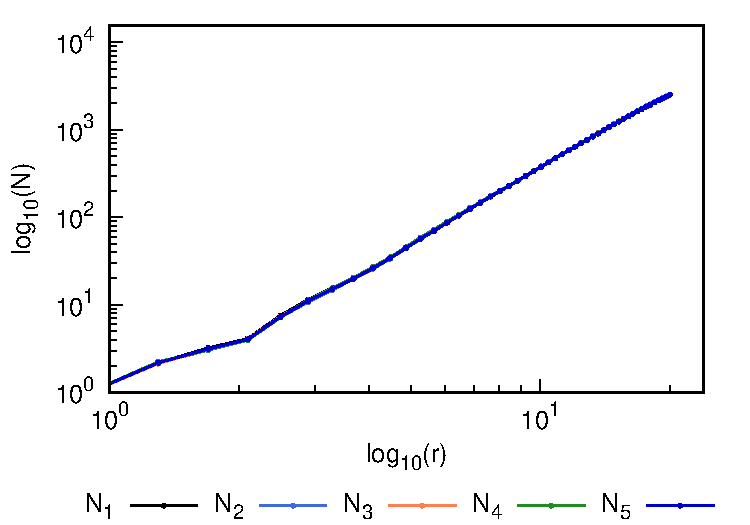
\includegraphics[width=\linewidth,page=1]{graphs/PDBs/Tubb4/TubMutA=200.pdf}
		\end{minipage}
		
		\caption{
			Gr\'{a}ficos de $log_{10}r$ vs $log_{10}M(r)$ correspondientes a una sola proteína \textit{Tubulina mutada} (treonina) despu\'{e}s de una din\'{a}mica molecular de 10 ns, estableciendo el número de medidas en  $A$ = 1 y 200 (izquierda a derecha). Donde $A = N_{means}$ y establece el número de medidas para obtener $\langle N(r_k) \rangle$, $\langle M(r_k) \rangle$ y $\langle Rg(r_k) \rangle$.}
		\label{fig:Tubs}
		\end{figure}
		
		

 	
 	\subsection{Paso 9 del diagrama de flujo general}
 		

 	\textbf{Determinación de la dimensión fractal.}  
 	Se asume un comportamiento de ley de potencias:
 	\begin{equation}
 		\langle M(r) \rangle \propto r^D
 	\end{equation}
 	Para encontrar $D$ se realiza una regresión lineal en escala logarítmica,
 	resolviendo el problema de mínimos cuadrados:
 
 		
 	\color{black}
 	
 	\section{Metodolog\'{i}a}
 	
 	El an\'{a}lisis fractal fue realizado tomando como punto de partida 9 de las 79 estructuras que se utilizaron anteriormente aplicando la restricci\'{o}n de la densidad de part\'{i}culas  promedio ($\rho_{p} \geq 0.034$) como criterio para determinar cuando un centro no es adecuado para realizar el conteo de part\'{i}culas y posteriormente, la cuantificaci\'{o}n de la masa como funci\'{o}n del radio de la esfera. Es decir, si una esfera de cierto radio centrada en alg\'{u}n punto tiene una $\rho_{p} < 0.34$, ser\'{a} altamente probable que la esfera intersecte en una zona que es considerada como un hueco de la prote\'{i}na. Por lo tanto, un centro con tales caracter\'{i}sticas podr\'{i}a ser descartado hasta que se encuentre otro centro adecuado (v\'{e}ase la figura \ref{fig:centrob}). Adem\'{a}s de lo anterior, se hizo uso del programa de din\'{a}mica molecular \textit{GROMACS}\cite{Lemkul2024, Abraham2015} que permite realizar simulaciones moleculares, con el fin de comparar diferentes estados de los sistemas proteicos. Los pasos esenciales de este proceso fueron los siguientes: (1) Preparaci\'{o}n de la topolog\'{i´}a del sistema. (2) Creaci\'{o}n de la caja y solvataci\'{o}n, (3) adici\'{o}n de iones para la neutralizaci\'{o}n de la carga, (4) minimizaci\'{o}n de la energ\'{i}a del sistema, (5) equilibrio del sistema, (6) simulaci\'{o}n de producci\'{o}n y (7) resultados.
 	
 	
 	
 	Hecho lo anterior, se extrajeron los respectivos archivos con formato \textit{PDB} en 
 	los siguientes pasos, para una comparaci\'{o}n posterior.
 	
 	\begin{enumerate}
 		\item Despu\'{e}s de adicionar \'{a}tomos de hidr\'{o}geno al sistema proteico. 
 		\item Tras finalizar el proceso de minimizaci\'{o}n de la energ\'{i}a.
 		\item Luego de completarse la etapa de equilibrio del sistema.
 		\item Completada la din\'{a}mica molecular durante un 1 ns.
 	\end{enumerate}
 	
 	
 	\subsection{Elecci\'{o}n de sistemas}
 	
 	\begin{table}[h!]
 		\centering
 		\begin{tabular}{llc}
 			\multicolumn{3}{c}{} \\ 
 			IdPDB & Nombre de prote\'{i}na & N\'{u}mero de \'{a}tomos \\
 			\hline
 			1a2b & Transformadora RHOA & 2831 \\
 			1a3n & Hemoglobina humana desoxidante cadena alfa & 8734 \\
 			1a8m & Factor de necr\'{o}sis tumoral alfa & 7104 \\
 			1a9w & Hemoglobina embrionaria cadena alfa & 8820 \\
 			1a52 & Receptor de estr\'{o}geno & 7765 \\
 			1auk & Arilsulfatasa A & 7086 \\
 			1b3e & Transferrina s\'{e}rica & 5037 \\
 			7khw & Translocon EspA & 131200 \\
 			11gs & Glutati\'{o}n s-transferasa & 6536 \\ 
 			\hline
 		\end{tabular}
 		\caption{Identificadores del \emph{Protein Data Bank} (PDB), nombre de la prote\'{i}na y n\'{u}mero de \'{a}tomos presentes en cada estructura.}
 		\label{Tabla:ids}
 	\end{table}
 	
 	
 	
 	La selecci\'{o}n de los sistemas se realiz\'{o} aleatoriamente bajo la condici\'{o}n de que contaran con la secuencia completa de amino\'{a}cidos, evitando componentes externos como ligandos o solventes que introducir\'{i}an ruido en el c\'{a}lculo de la dimensi\'{o}n fractal intr\'{i}nseca de las prote\'{i}nas. Los sistemas analizados se listan en la Tabla \ref{Tabla:ids}.
 
	
	
	
	\subsection{Determinaci\'{o}n de $M(r)$}
	
	Se calcul\'{o} la masa promedio de las part\'{i}culas contenidas dentro de esferas de radio $r_i$, definida como $\bar{M}(r_i)$. 
	Para llevar a cabo este an\'{a}lisis, se us\'{o} la herramienta \textit{molfractaldim}. ajustando dos par\'{a}metros clave: El primero define cu\'{a}ntos valores se promedian para obtener el valor de $\bar{M}(r_i)$ y el segundo, determina cu\'{a}ntos radios $r_{i}$ se toman para la medici\'{o}n. Donde: 
	
	\begin{itemize}
		\item $r_{i}$ es el radio de una esfera.
		\item $\bar M(r_{i})$ es la masa promedio de las part\'{i}culas contenidas dentro la esfera de radio $r_{i}$.
	\end{itemize}
	
	
	
	Ambos valores se fijaron en 200 para asegurar resultados representativos y detallados. Este procedimiento se aplic\'{o} en cada uno de los archivos listados en la Tabla~\ref{Tabla:ids}, correspondientes a los pasos descritos en la secci\'{o}n \ref{met}.
	
	
	\begin{comment}
		Determinaci\'{o}n de la masa promedio de las part\'{i}culas $\bar M(r_{i})$ dentro de cada radio $r_{i}$.Donde:
		
		\begin{itemize}
			\item $r_{i}$ es el radio de una esfera.
			\item $\bar M(r_{i})$ es la masa promedio de las part\'{i}culas promedio contenidas dentro una esfera de radio $r$.
		\end{itemize}
		
		A partir del programa \textit{molmassfractaldim} usando las restriciones $-a$ y $-n$ que modifican el n\'{u}mero promedios para  $M(r)$ y establecen el n\'{u}mero de radios para $M(r)$ vs $r$.  Este procedimiento se aplic\'{o} a cada uno de los 9 archivos listados en la Tabla \ref{Tabla:ids}, correspondientes a cada paso descrito en la metodolog\'{i´}a. 
	\end{comment}
	
	
	\subsection{An\'{a}lisis multifractal}
	
	Se realiz\'{o} un an\'{a}lisis multifractal sobre los datos extra\'{i}dos del paso anterior, para calcular la \textbf{dimensi\'{o}n fractal} $D$, donde el \textbf{exponente de escala} $b$  relaciona la masa  promedio $\bar{M}(r_i)$ con el radio $r_{i}$ mediante:
	\begin{equation}
		\bar{M}(r_i) \sim r_{i}^b
	\end{equation}
	
	Para un sistema multifractal, $b$ var\'{i}a seg\'{u}n la escala espacial, reflejando heterogeneidad en la distribuci\'{o}n de masa.
	\begin{itemize}
		\item \textbf{Coeficiente de determinaci\'{o}n $R^{2}$}: \\ Es una medida de correlaci\'{o}n lineal entre $log_{10}M(r)$ y $log_{10}r$.
		\item \textbf{Pendiente $b$}:
		\begin{itemize}
			\item Si $b$ muestra un \'{u}nico valor en el intervalo general 1 - 20$\textup{\r{A}}$: Existe un comportamiento monofractal (estructura homog\'{e}nea).
			\item Si $b$  tiene distintos valores en el intervalo general de 1 - 20$\textup{\r{A}}$: Existe multifractalidad (estructura heterog\'{e}nea).
		\end{itemize}
	\end{itemize}
	
	A continuaci\'{o}n, se llevaron a cabo m\'{u}ltiples regresiones lineales sobre cada archivo de datos num\'{e}ricos, en intervalos donde era altamente probable encontrar distintos valores de dimensi\'{o}n fractal. Estos intervalos fueron: 1 a 2~$\textup{\r{A}}$, 2 a 6~$\textup{\r{A}}$ y 6 a 20~$\textup{\r{A}}$ \cite{Enright2005, Liu2020}.	
	
	
	
	La selecci\'on del intervalo 2--6~$\textup{\r{A}}$ utilizado para la medici\'on o implementaci\'on de ajustes lineales en el an\'alisis multifractal tiene su origen en el di\'ametro promedio de los amino\'acidos ($d_p$) reportado por Siyuan Liu \textit{et al.} \citen{Liu2020} siendo $d_p \approx$ 4,188 $\textup{\r{A}}$. Posteriomente, la elecci\'{o}n de los intervalos parciales 1--2~$\textup{\r{A}}$ y 6--20~$\textup{\r{A}}$ fueron elegidos heur\'{i}sticamente, observando las gr\'{a}ficas de $log_{10}r$ vs $log_{10}M(r)$ de cada prote\'{i}na de la Tabla \ref{Tabla:ids}.
	
	\begin{figure}[H]
		\subsection*{Caso particular de estudio: tubulina nativa y mutada}	
		\hspace{-0.3cm} 
		\begin{minipage}{0.49\textwidth}
			\centering
			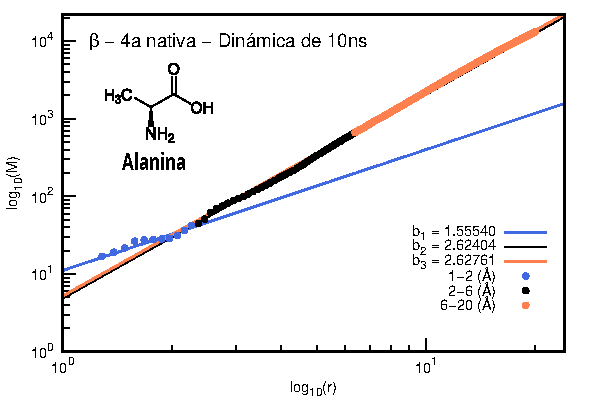
\includegraphics[width=\linewidth,page=1]{graphs/PDBs/Tubb4/TubNat10ns.pdf}
		\end{minipage}
		\hspace{0.2cm}
		\begin{minipage}{0.49\textwidth}
			\centering
			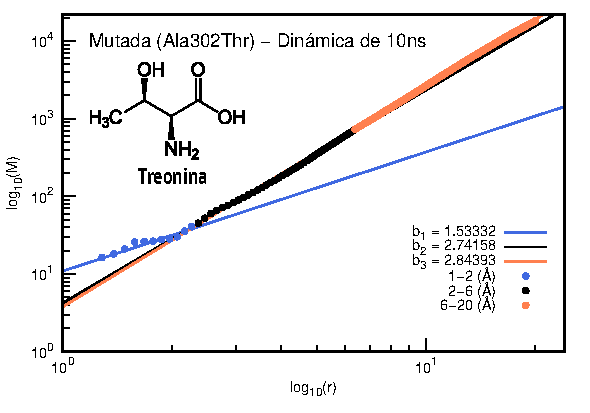
\includegraphics[width=\linewidth,page=1]{graphs/PDBs/Tubb4/TubMut10ns.pdf}
		\end{minipage}
		
		
		\caption{
			Gr\'{a}ficos de $log_{10}r$ vs $log_{10}M(r)$ correspondientes a dos prote\'{i}nas diferentes: \textit{Tubulina nativa} (alanina) y \textit{Tubulina mutada} (treonina) despu\'{e}s de una din\'{a}mica molecular de 10 ns. Los valores de $b$ en cada gr\'{a}fica representan la dimensi\'{o}n fractal de masa en los intervalos 1 a 2~$\textup{\r{A}}$, 2 a 6~$\textup{\r{A}}$ y 6 a 20~$\textup{\r{A}}$.}
		\label{fig:Tubs}
	\end{figure}
	
	
	
	
	\begin{figure}[H]
		\subsection*{Efecto de iones en la dimensi\'{o}n fractal}	
		\centering
		\begin{subfigure}{0.49\textwidth}
			\centering
			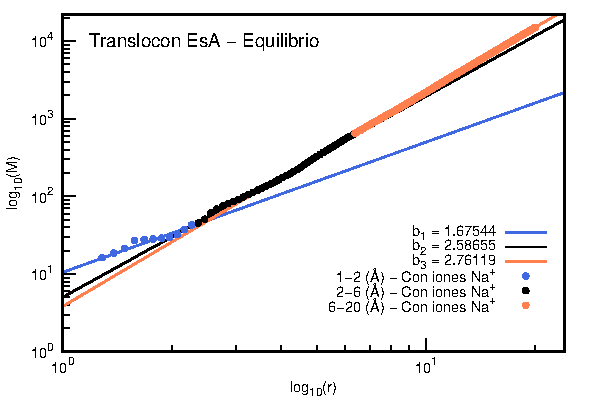
\includegraphics[width=\linewidth,page=1]{graphs/PDBs/7khw/ions/7khwEq-wions.pdf}
			\caption{(1)}
		\end{subfigure}
		\hfill
		\begin{subfigure}{0.49\textwidth}
			\centering
			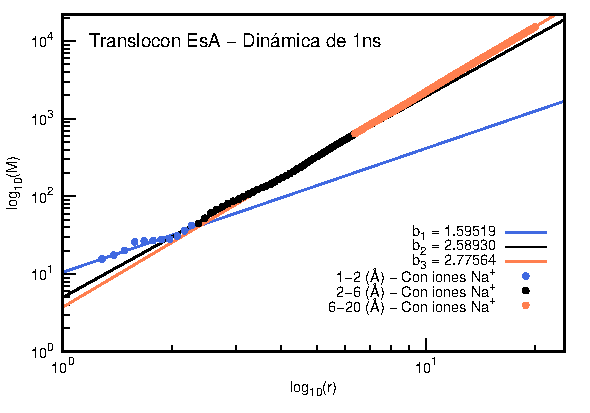
\includegraphics[width=\linewidth,page=1]{graphs/PDBs/7khw/ions/7khw1ns-wions.pdf}
			\caption{(2)}
		\end{subfigure}
		\caption{Gr\'{a}ficos de $log_{10}r$ vs $log_{10}M(r)$ correspondientes a dos etapas de procesamiento de la octava prote\'{i}na \textit{Translocon EsA} (con iones Na$^{+}$ en su estructura) de la Tabla \ref{Tabla:ids} despu\'{e}s de (1) equilibrar el sistema bajo condiciones termodin\'{a}micas controladas y (2) de una din\'{a}mica molecular de 1 ns. Los valores de $b$ en cada gr\'{a}fica representan la dimensi\'{o}n fractal de masa en los intervalos 1 a 2~$\textup{\r{A}}$, 2 a 6~$\textup{\r{A}}$ y 6 a 20~$\textup{\r{A}}$.}
		\label{fig:7khw-wions}
	\end{figure}
	
	
	\begin{figure}[H]
		\centering
		\begin{subfigure}{0.49\textwidth}
			\centering
			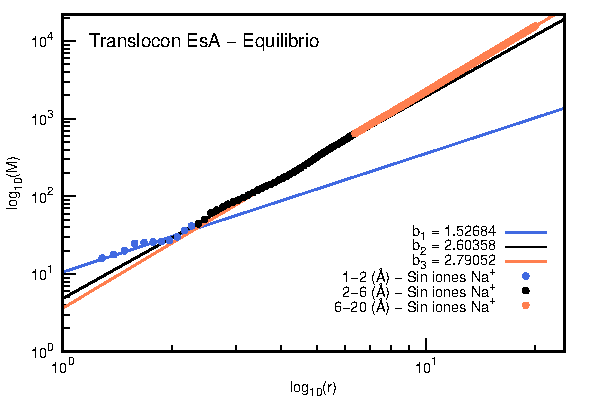
\includegraphics[width=\linewidth,page=1]{graphs/PDBs/7khw/ions/7khwEq-oions.pdf}
			\caption{(1)}
		\end{subfigure}
		\hfill
		\begin{subfigure}{0.49\textwidth}
			\centering
			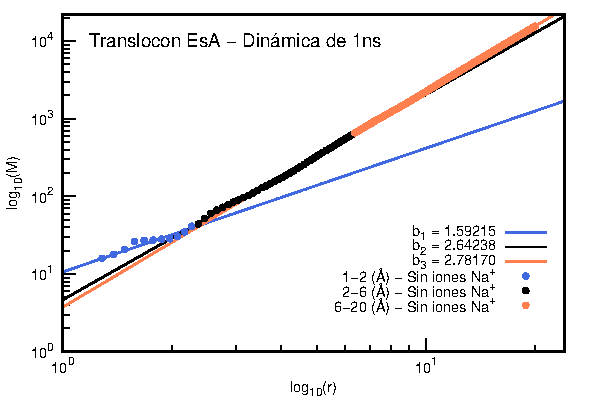
\includegraphics[width=\linewidth,page=1]{graphs/PDBs/7khw/ions/7khw1ns-oions.pdf}
			\caption{(2)}
		\end{subfigure}
		\caption{Gr\'{a}ficos de $log_{10}r$ vs $log_{10}M(r)$ correspondientes a dos etapas de procesamiento de la octava prote\'{i}na \textit{Translocon EsA} (sin iones Na$^{+}$ en su estructura) de la Tabla \ref{Tabla:ids} despu\'{e}s de (1) equilibrar el sistema bajo condiciones termodin\'{a}micas controladas y (2) de una din\'{a}mica molecular de 1 ns. Los valores de $b$ en cada gr\'{a}fica representan la dimensi\'{o}n fractal de masa en los intervalos 1 a 2~$\textup{\r{A}}$, 2 a 6~$\textup{\r{A}}$ y 6 a 20~$\textup{\r{A}}$.}
		\label{fig:7khw-oions}
	\end{figure}
	
	\begin{table}[H]
		\centering
		\begin{tabular}{lllSS}
			\toprule
			\multicolumn{5}{c}{\textbf{Translocon EsA}} \\
			\midrule
			\textbf{Estado de la prote\'{i}na} & \textbf{Etapa} & \textbf{Intervalo (\AA)} & \textbf{$R^{2}$} & \textbf{Pendiente ($b$)} \\
			\midrule
			\multirow{6}{*}{\centering Con Na$^{+}$}
			&            & 1-2 & 0.933264 & 1.67544 \\
			& Equilibrio & 2-6 & 0.997049 & 2.58655 \\
			&            & 6-20 & 0.999965 & 2.76119 \\
			\cmidrule(lr){2-5}
			&                    & 1-2 & 0.938494 & 1.59519 \\
			& Din\'{a}mica (1ns) & 2-6 & 0.997471 & 2.5893 \\
			&                    & 6-20 & 0.999977 & 2.77564 \\
			
			\cmidrule(lr){2-5}
			\multirow{6}{*}{\centering Sin Na$^{+}$}
			&            & 1-2 & 0.930791 & 1.52684 \\
			& Equilibrio & 2-6 & 0.996961 & 2.60358 \\
			&            & 6-20 & 0.999988 & 2.79052 \\
			\cmidrule(lr){2-5}
			&                    & 1-2 & 0.929409 & 1.59215 \\
			& Din\'{a}mica (1ns) & 2-6 & 0.99807 & 2.64238 \\
			&                    & 6-20 & 0.999938 & 2.78170 \\
			\bottomrule
		\end{tabular}
		\caption{Datos de regresi\'{o}n lineal de $log_{10}r$ vs $log_{10}M(r)$ de las Figuras \ref{fig:7khw-wions} y \ref{fig:7khw-oions}.}
		\label{tab:tab-7khw}
	\end{table}
	
	
	
	\begin{figure}[H]
		\subsection*{Dimensiones fractales en distintas etapas}	
		\centering
		\begin{subfigure}{0.49\textwidth}
			\centering
			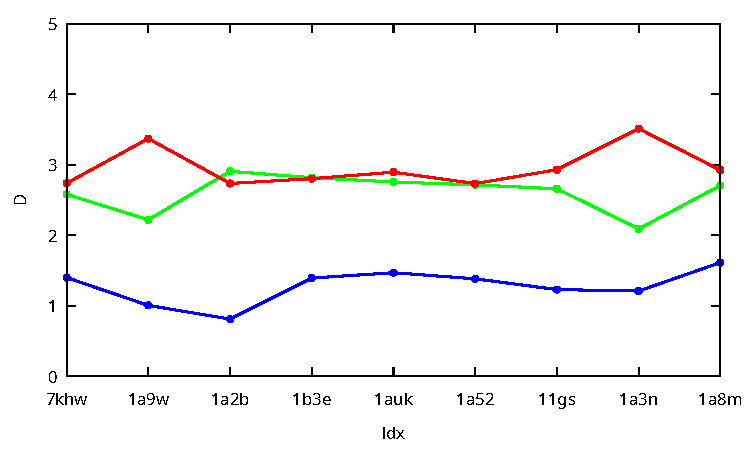
\includegraphics[width=\linewidth,page=1]{graphs/PDBs/Dvsldx/DvsaddH.pdf}
			\caption{(1)}
		\end{subfigure}
		\hfill
		\begin{subfigure}{0.49\textwidth}
			\centering
			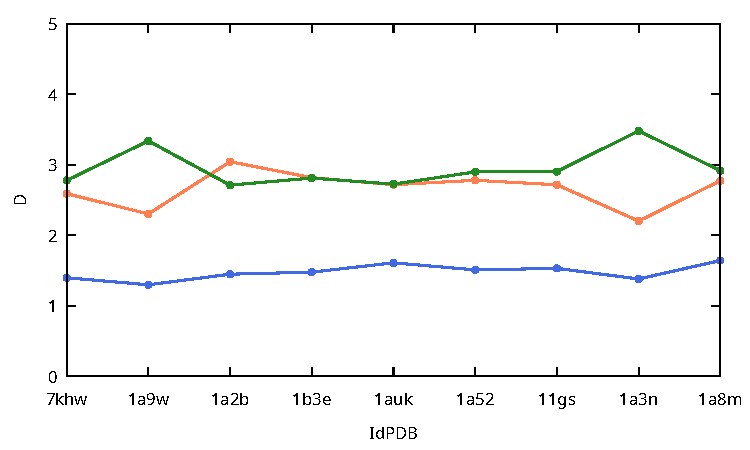
\includegraphics[width=\linewidth,page=1]{graphs/PDBs/Dvsldx/DvsEm.pdf}
			\caption{(2)}
		\end{subfigure}
		
		\vspace{0.3cm}
		
		\begin{subfigure}{0.49\textwidth}
			\centering
			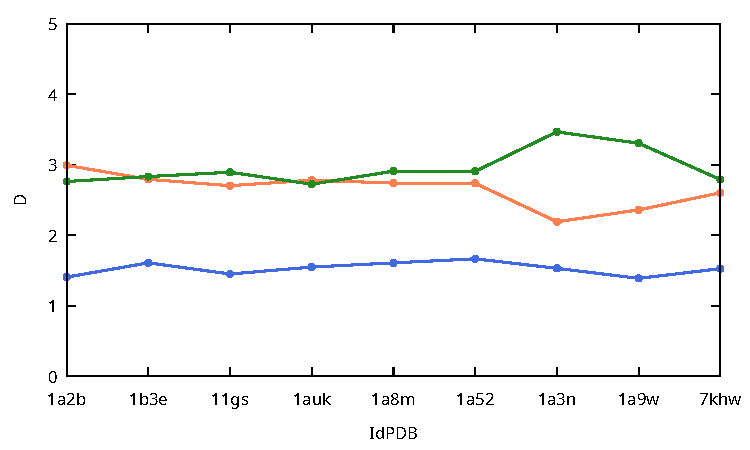
\includegraphics[width=\linewidth,page=1]{graphs/PDBs/Dvsldx/DvsEq.pdf}
			\caption{(3)}
		\end{subfigure}
		\hfill
		\begin{subfigure}{0.49\textwidth}
			\centering
			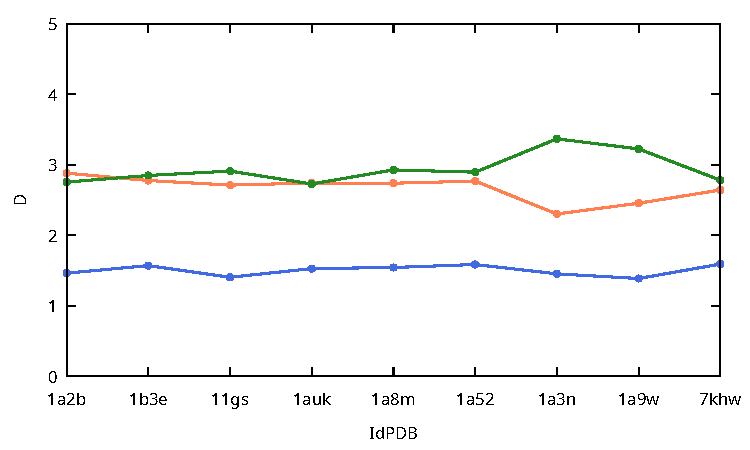
\includegraphics[width=\linewidth,page=1]{graphs/PDBs/Dvsldx/DvsDm.pdf}
			\caption{(4)}
		\end{subfigure}
		
		\caption{Valores de dimensi\'{o}n fractal de masa $D$ vs \'{i}ndice de prote\'{i}nas para las prote\'{i}nas ilustradas en la tabla \ref{Tabla:ids}, correspondientes a cuatro etapas de procesamiento: (1) Adici\'{o}n de \'{a}tomos de hidr\'{o}geno al sistema proteico, (2) al minimizar la energ\'{i´}a de la estructura molecular, (3) equilibrando el sistema bajo condiciones termodin\'{a}micas controladas y (4) despu\'{e}s de una din\'{a}mica molecular de 1 ns. Las líneas azules, verdes y rojas representan $D$ en los intervalos de 1 a 2~$\textup{\r{A}}$, 2 a 6~$\textup{\r{A}}$ y 6 a 20~$\textup{\r{A}}$, respectivamente.}
		\label{fig:Df-general}
	\end{figure}
	
	
	
	%\section{Discusi\'{o}n de resultados}	
	
	En la Figura \ref{fig:Df-general}, las prote\'{i}nas \textit{Hemoglobin} (1a9w y 1a3n) exhiben valores de dimensi\'{o}n fractal $D \approx 3.5$ en todas las etapas, con una reducci\'{o}n  ($\Delta D < 0.2$) posterior al equilibrio termodin\'{a}mico y una din\'{a}mica molecular de 1ns. El valor $D \approx 3.5$  es contraintuitivo, pero podr\'{i}a deberse a que nuestro estudio se ha enfocado en analizar la dimensi\'{o}n fractal de masa (se toman en cuenta las masas promedio de los \'{a}tomos en la medida) y no la dimensi\'{o}n fractal del número de part\'{i}culas (no depende de la masa promedio de las part\'{i}culas presentes en la estructura proteica). Adem\'{a}s, se identifica una correlaci\'{o}n inversa (\emph{relaci\'{o}n tipo espejo}) entre los intervalos 2--6~$\textup{\r{A}}$ y 6--20~$\textup{\r{A}}$, particularmente marcada durante la etapa de equilibrio del sistema.
	
	Este comportamiento sugiere la coexistencia de al menos, dos dimensiones fractales diferenciadas en cada prote\'{i}na en los intervalos de 1--2~$\textup{\r{A}}$ y 2--6~$\textup{\r{A}}$ persistentes en todas las fases de simulaci\'{o}n. La variaci\'{o}n de $D$ evidencia un \textbf{comportamiento multifractal}, donde la dimensi\'{o}n fractal evolucionan progresivamente desde organizaciones locales hasta globales. Estos hallazgos confirman que cada etapa computacional (adicci\'{o}n, minimizaci\'{o}n, equilibrio y din\'{a}mica molecular) inciden significativamente en la reconfiguraci\'{o}n de la dimensi\'{o}n fractal proteica. Adem\'{a}s, algunos sistemas proteicos tienen una estructura cuaternaria, es decir, para llevar a cabo su función requieren de cuatro mon\'{o}meros perfectamente plegados que se unen por interacciones no covalentes para adquirir un car\'{a}cter funcional. Esto sugiere que la medición podría ser lo suficientemente sensible como para detectar niveles superiores de organización proteica.
	
	
	
	
	\subsection*{Caso particular de estudio: tubulinas}
	
	La comparaci\'{o}n presentada en la Figura~\ref{fig:Tubs} examina dos variantes estructurales:
	\begin{itemize}
		\item Prote\'{i}na nativa: 6,812 \'{a}tomos (estructura de referencia).
		\item Variante mutada: 6,816 \'{a}tomos (reemplazo de un residuo aminoac\'{i}dico).
	\end{itemize}
	
	Los resultados obtenidos demostraron diferencias en las pendientes de la regresi\'{o}n lineal analizadas espec\'{i}ficamente en la etapa final del procesamiento (despu\'{e}s de una din\'{a}mica molecular de 10 ns). Esta diferencia estructural se observa a pesar de la alta similitud global entre ambas variantes.
	La detecci\'{o}n de estas diferencias sutiles valida la sensibilidad del m\'{e}todo propuesto para discriminar modificaciones estructurales m\'{i}nimas.
	
	
	
	\subsection*{Efecto de iones}
	
	En las Figuras \ref{fig:7khw-wions} y \ref{fig:7khw-oions}, se compara la distribuci\'{o}n de masa de la prote\'{i}na \textit{Translocon EsA} (7khw) en dos etapas: Tras el equilibrio estructural y luego de una din\'{a}mica molecular de 1~ns. La Figura \ref{fig:7khw-wions} considera la estructura proteica con iones presentes, revelando tres pendientes en la regresi\'{o}n $log_{10}r$ vs $log_{10}M(r)$, lo que sugiere una multifractalidad en 3 intervalos. Sin embargo, en la Figura \ref{fig:7khw-oions}, 250 iones de sodio que no pertenec\'{i}an a la estructura intr\'{i}nseca de la prote\'{i}na fueron eliminados, con el fin de validar la reproducibilidad de los resultados. Sorprendentemente, en el \'{u}ltimo caso solo se observaron dos pendientes, aunque la estructura original conten\'{i}a  un excedente de 250 \'{a}tomos de sodio (aproximadamente el 0.19\% comparado con los 131,200 átomos presentes en la estructura proteica). Por lo tanto, esta comparaci\'{o}n evidenci\'{o} que la estimaci\'{o}n de dimensi\'{o}n fractal de masa es sensible a modificaciones estructurales m\'{i}nimas. Estos resultados respaldan el uso potencial de dicha medida como herramienta de caracterizaci\'{o}n estructural en prote\'{i}nas. 
 
 	
 
		\begin{figure}[H]
			\subsection*{IdPDB:1a2b}	
			\hspace{-0.3cm} 
			\begin{subfigure}{0.49\textwidth}
				\centering
				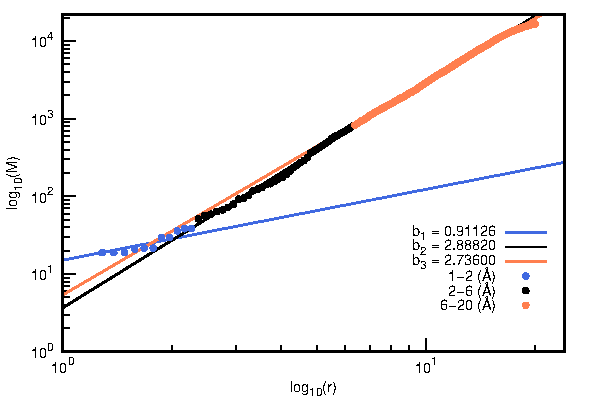
\includegraphics[width=\linewidth,page=1]{graphs/PDBs/1a2b/1a2baddH.pdf}
				\caption{(1)}
			\end{subfigure}
			\hspace{0.2cm}
			\begin{subfigure}{0.49\textwidth}
				\centering
				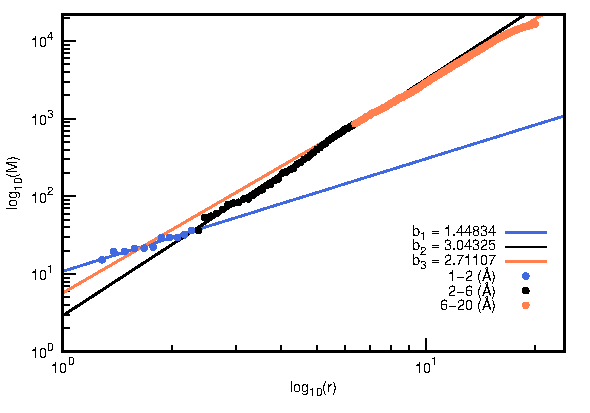
\includegraphics[width=\linewidth,page=1]{graphs/PDBs/1a2b/1a2bEm.pdf}
				\caption{(2)}
			\end{subfigure}
			
			\vspace{0cm} % Espacio entre filas
			
			\hspace{-0.3cm} 
			\begin{subfigure}{0.49\textwidth}
				\centering
				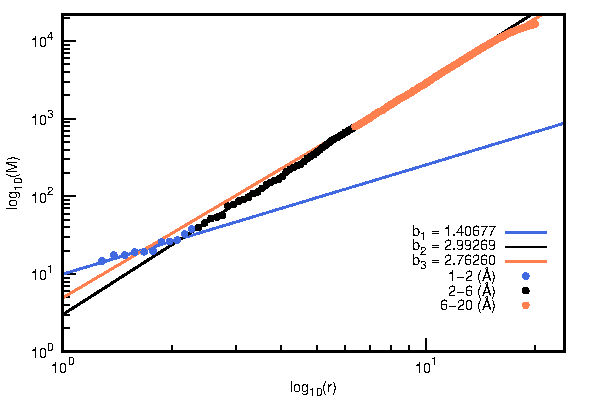
\includegraphics[width=\linewidth,page=1]{graphs/PDBs/1a2b/1a2bEq.pdf}
				\caption{(3)}
			\end{subfigure}
			\hspace{0.2cm}
			\begin{subfigure}{0.49\textwidth} % M\'{a}s ancho para centrar
				\centering
				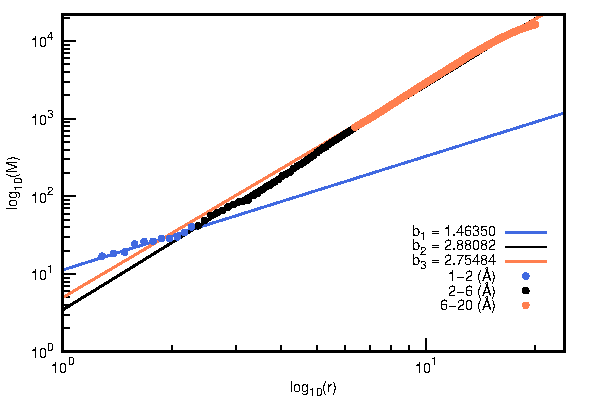
\includegraphics[width=\linewidth,page=1]{graphs/PDBs/1a2b/1a2b1ns.pdf}
				\caption{(4)}
			\end{subfigure}
			
			\caption{
				Regresiones lineales de $log_{10}r$ vs $log_{10}M(r)$ correspondiente a cuatro etapas de procesamiento de la primera prote\'{i}na con \textit{IdPDB:1a2b} de la Tabla \ref{Tabla:ids}: (1) Adici\'{o}n de \'{a}tomos de hidr\'{o}geno al sistema proteico; (2) al minimizar la energ\'{i´}a de la estructura molecular; (3) equilibrando el sistema bajo condiciones termodin\'{a}micas controladas; y (4) despu\'{e}s de una din\'{a}mica molecular de 1 ns.}
			\label{fig:1a2b}
		\end{figure}
		
		\begin{figure}[H]
			\subsection*{IdPDB:1a3n}
			
			\hspace{-0.3cm} 
			\begin{subfigure}{0.49\textwidth}
				\centering
				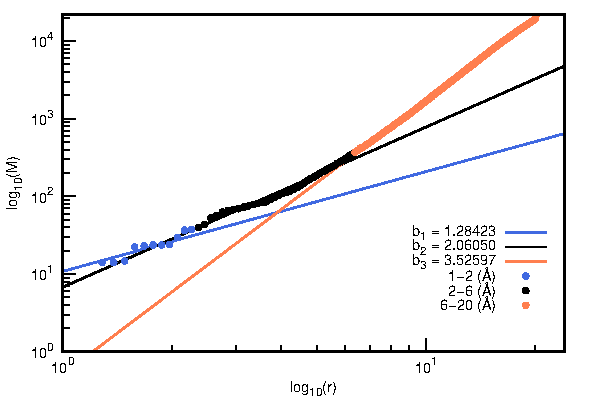
\includegraphics[width=\linewidth,page=1]{graphs/PDBs/1a3n/1a3naddH.pdf}
				\caption{(1)}
			\end{subfigure}
			\hspace{0.2cm}
			\begin{subfigure}{0.49\textwidth}
				\centering
				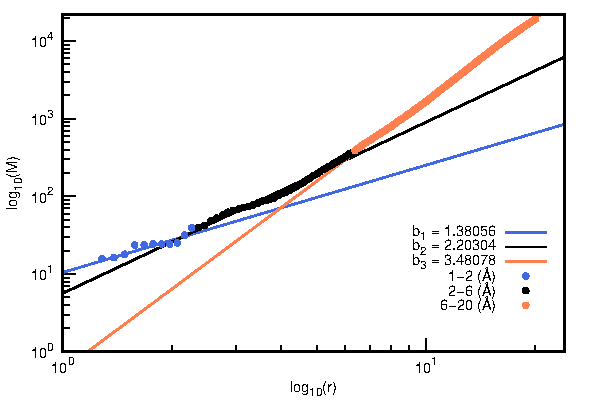
\includegraphics[width=\linewidth,page=1]{graphs/PDBs/1a3n/1a3nEm.pdf}
				\caption{(2)}
			\end{subfigure}
			
			\vspace{0cm} % Espacio entre filas
			
			\hspace{-0.3cm} 
			\begin{subfigure}{0.49\textwidth}
				\centering
				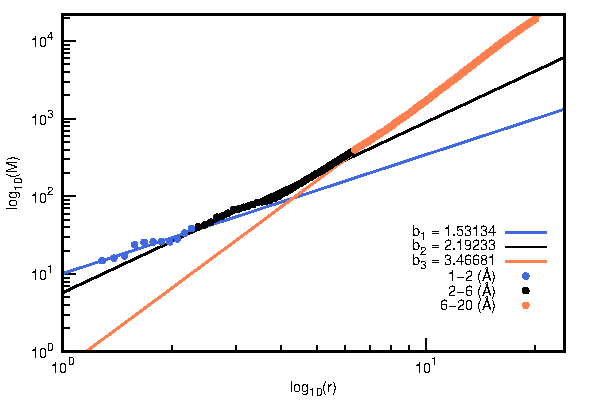
\includegraphics[width=\linewidth,page=1]{graphs/PDBs/1a3n/1a3nEq.pdf}
				\caption{(3)}
			\end{subfigure}
			\hspace{0.2cm}
			\begin{subfigure}{0.49\textwidth} % M\'{a}s ancho para centrar
				\centering
				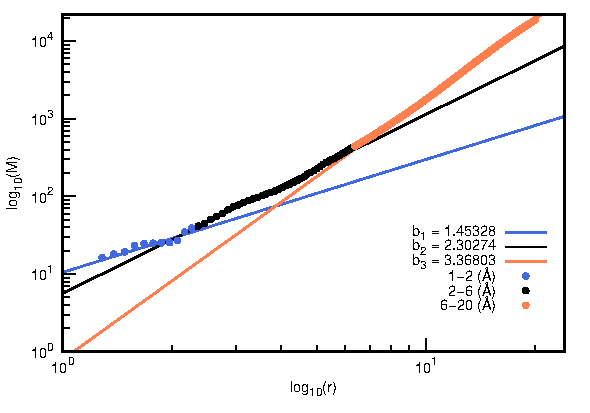
\includegraphics[width=\linewidth,page=1]{graphs/PDBs/1a3n/1a3n1ns.pdf}
				\caption{(4)}
			\end{subfigure}
			\caption{Regresiones lineales de $log_{10}r$ vs $log_{10}M(r)$ correspondiente a cuatro etapas de procesamiento de la segunda prote\'{i}na con \textit{IdPDB:1a3n} de la Tabla \ref{Tabla:ids}: (1) Adici\'{o}n de \'{a}tomos de hidr\'{o}geno al sistema proteico; (2) al minimizar la energ\'{i´}a de la estructura molecular; (3) equilibrando el sistema bajo condiciones termodin\'{a}micas controladas; y (4) despu\'{e}s de una din\'{a}mica molecular de 1 ns.}
			\label{fig:1a3n}
		\end{figure}
		
		\begin{figure}[H]
			\subsection*{IdPDB:1a8m}
			
			\hspace{-0.3cm} 
			\begin{subfigure}{0.49\textwidth}
				\centering
				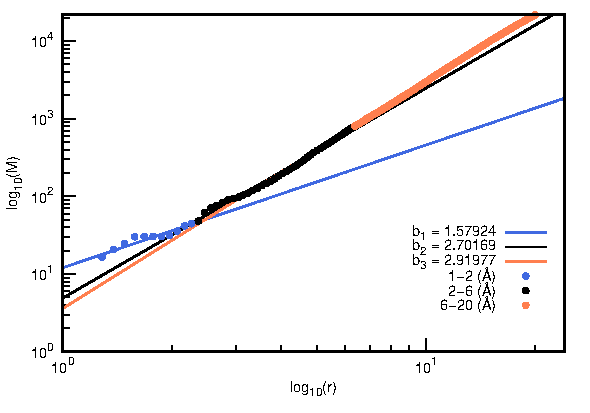
\includegraphics[width=\linewidth,page=1]{graphs/PDBs/1a8m/1a8maddH.pdf}
				\caption{(1)}
			\end{subfigure}
			\hspace{0.2cm}
			\begin{subfigure}{0.49\textwidth}
				\centering
				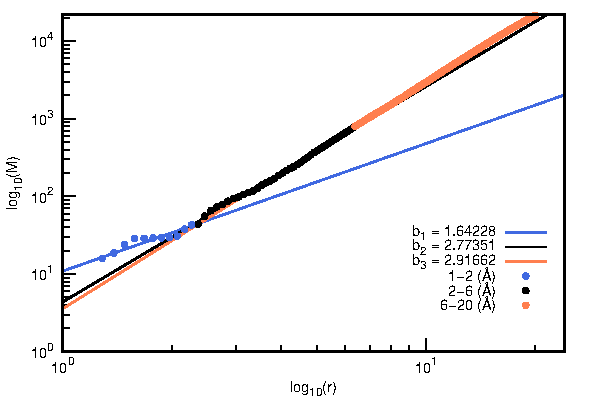
\includegraphics[width=\linewidth,page=1]{graphs/PDBs/1a8m/1a8mEm.pdf}
				\caption{(2)}
			\end{subfigure}
			
			\vspace{0cm} % Espacio entre filas
			
			\hspace{-0.3cm} 
			\begin{subfigure}{0.49\textwidth}
				\centering
				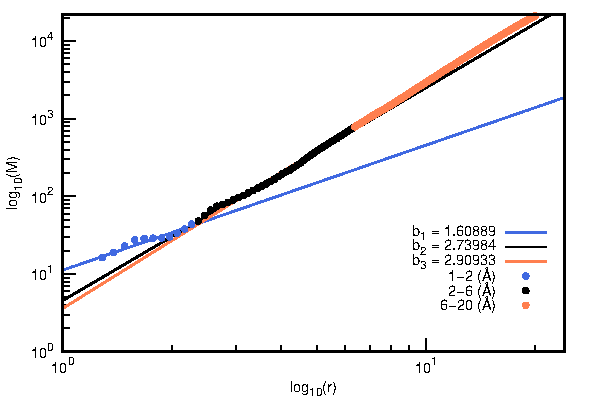
\includegraphics[width=\linewidth,page=1]{graphs/PDBs/1a8m/1a8mEq.pdf}
				\caption{(3)}
			\end{subfigure}
			\hspace{0.2cm}
			\begin{subfigure}{0.49\textwidth} % M\'{a}s ancho para centrar
				\centering
				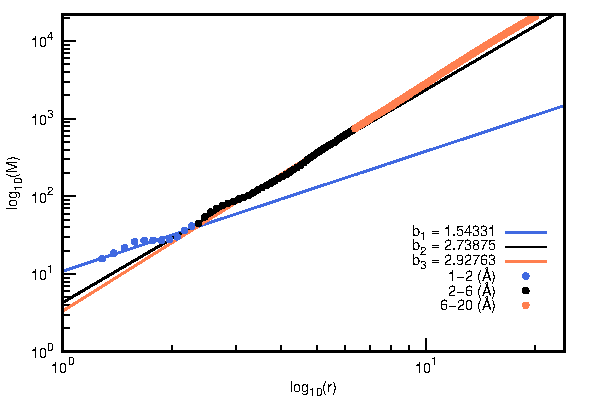
\includegraphics[width=\linewidth,page=1]{graphs/PDBs/1a8m/1a8m1ns.pdf}
				\caption{(4)}
			\end{subfigure}
			\caption{Regresiones lineales de $log_{10}r$ vs $log_{10}M(r)$ correspondiente a cuatro etapas de procesamiento de la cuarta prote\'{i}na con \textit{IdPDB:1a8m} de la Tabla \ref{Tabla:ids}: (1) Adici\'{o}n de \'{a}tomos de hidr\'{o}geno al sistema proteico; (2) al minimizar la energ\'{i´}a de la estructura molecular; (3) equilibrando el sistema bajo condiciones termodin\'{a}micas controladas; y (4) despu\'{e}s de una din\'{a}mica molecular de 1 ns.}
			\label{fig:1a8m}
		\end{figure}
		
		
		\begin{figure}[H]
			\subsection*{IdPDB:1a9w}
			
			\hspace{-0.3cm} 
			\begin{subfigure}{0.49\textwidth}
				\centering
				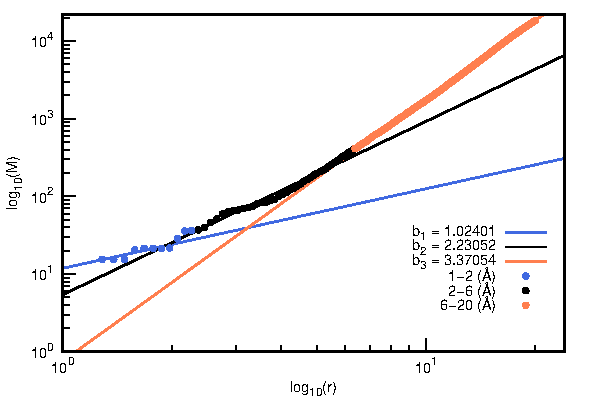
\includegraphics[width=\linewidth,page=1]{graphs/PDBs/1a9w/1a9waddH.pdf}
				\caption{(1)}
			\end{subfigure}
			\hspace{0.2cm}
			\begin{subfigure}{0.49\textwidth}
				\centering
				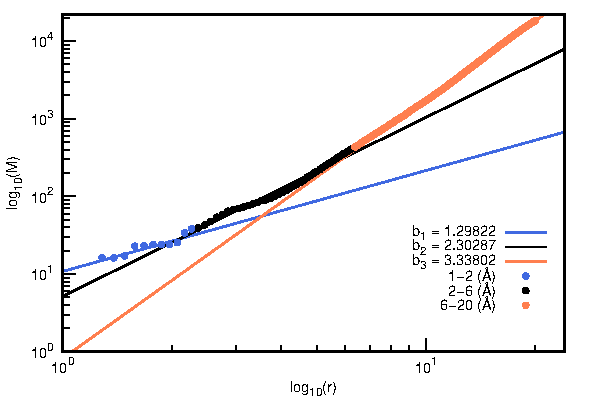
\includegraphics[width=\linewidth,page=1]{graphs/PDBs/1a9w/1a9wEm.pdf}
				\caption{(2)}
			\end{subfigure}
			
			\vspace{0cm} % Espacio entre filas
			
			\hspace{-0.3cm} 
			\begin{subfigure}{0.49\textwidth}
				\centering
				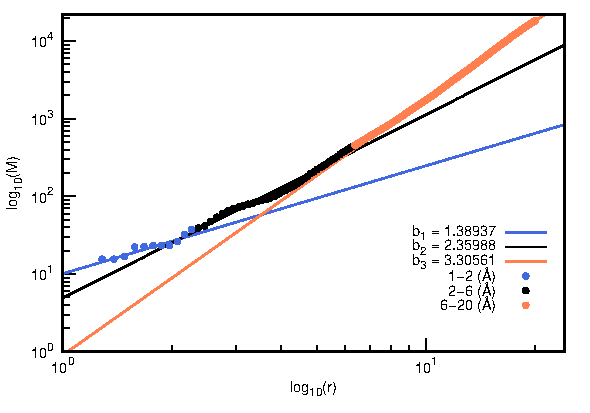
\includegraphics[width=\linewidth,page=1]{graphs/PDBs/1a9w/1a9wEq.pdf}
				\caption{(3)}
			\end{subfigure}
			\hspace{0.2cm}
			\begin{subfigure}{0.49\textwidth} % M\'{a}s ancho para centrar
				\centering
				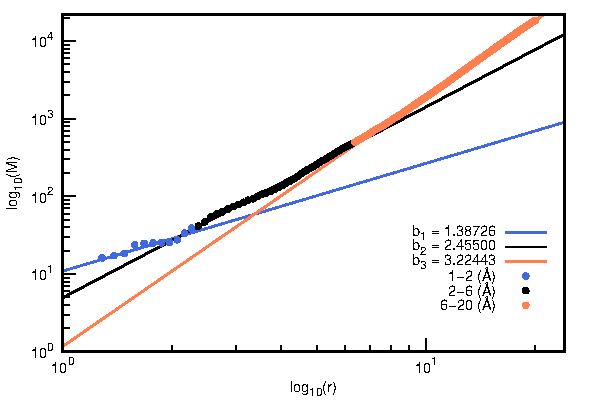
\includegraphics[width=\linewidth,page=1]{graphs/PDBs/1a9w/1a9w1ns.pdf}
				\caption{(4)}
			\end{subfigure}
			\caption{Regresiones lineales de $log_{10}r$ vs $log_{10}M(r)$ correspondiente a cuatro etapas de procesamiento de la quinta prote\'{i}na con \textit{IdPDB:1a9w} de la Tabla \ref{Tabla:ids}: (1) Adici\'{o}n de \'{a}tomos de hidr\'{o}geno al sistema proteico; (2) al minimizar la energ\'{i´}a de la estructura molecular; (3) equilibrando el sistema bajo condiciones termodin\'{a}micas controladas; y (4) despu\'{e}s de una din\'{a}mica molecular de 1 ns.}
			\label{fig:1a9w}
		\end{figure}
		
		\begin{figure}[H]
			\subsection*{IdPDB:1a52}
			
			\hspace{-0.3cm} 
			\begin{subfigure}{0.49\textwidth}
				\centering
				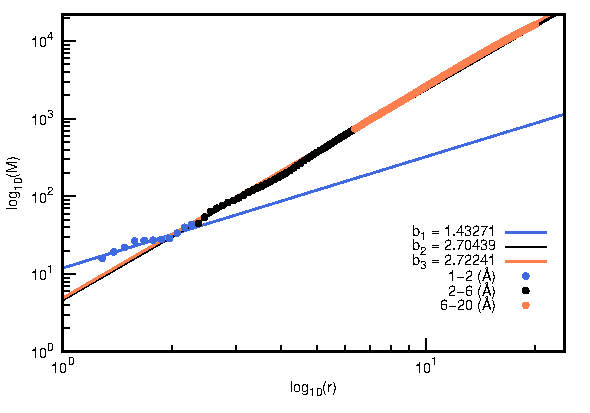
\includegraphics[width=\linewidth,page=1]{graphs/PDBs/1a52/1a52addH.pdf}
				\caption{(1)}
			\end{subfigure}
			\hspace{0.2cm}
			\begin{subfigure}{0.49\textwidth}
				\centering
				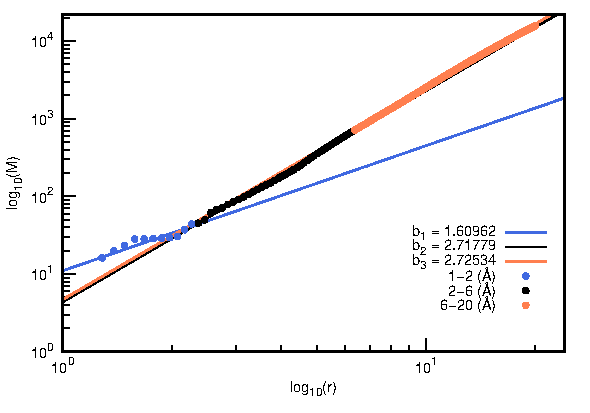
\includegraphics[width=\linewidth,page=1]{graphs/PDBs/1a52/1a52Em.pdf}
				\caption{(2)}
			\end{subfigure}
			
			\vspace{0cm} % Espacio entre filas
			
			\hspace{-0.3cm} 
			\begin{subfigure}{0.49\textwidth}
				\centering
				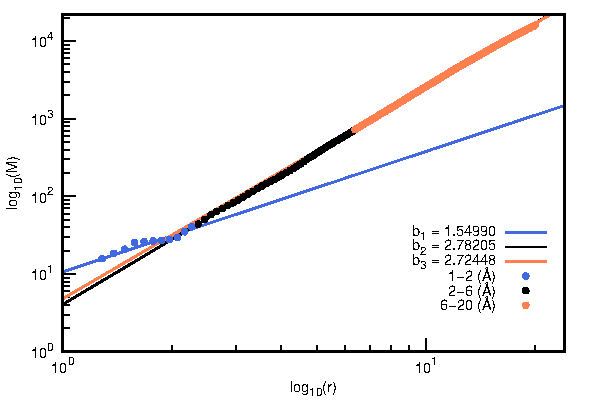
\includegraphics[width=\linewidth,page=1]{graphs/PDBs/1a52/1a52Eq.pdf}
				\caption{(3)}
			\end{subfigure}
			\hspace{0.2cm}
			\begin{subfigure}{0.49\textwidth} % M\'{a}s ancho para centrar
				\centering
				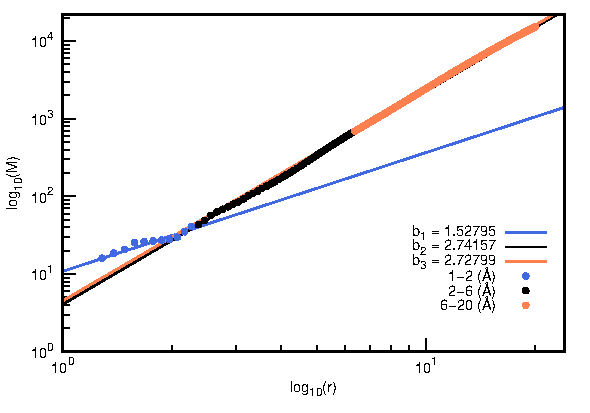
\includegraphics[width=\linewidth,page=1]{graphs/PDBs/1a52/1a521ns.pdf}
				\caption{(4)}
			\end{subfigure}
			\caption{Regresiones lineales de $log_{10}r$ vs $log_{10}M(r)$ correspondiente a cuatro etapas de procesamiento de la tercera prote\'{i}na con \textit{IdPDB:1a52} de la Tabla \ref{Tabla:ids}: (1) Adici\'{o}n de \'{a}tomos de hidr\'{o}geno al sistema proteico; (2) al minimizar la energ\'{i´}a de la estructura molecular; (3) equilibrando el sistema bajo condiciones termodin\'{a}micas controladas; y (4) despu\'{e}s de una din\'{a}mica molecular de 1 ns.}
			\label{fig:1a52}
		\end{figure}
		
		
		\begin{figure}[H]
			\subsection*{IdPDB:1auk}
			\hspace{-0.3cm} 
			\begin{subfigure}{0.49\textwidth}
				\centering
				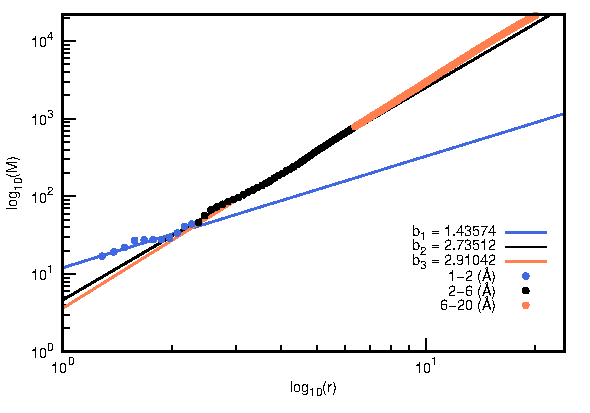
\includegraphics[width=\linewidth,page=1]{graphs/PDBs/1auk/1aukaddH.pdf}
				\caption{(1)}
			\end{subfigure}
			\hspace{0.2cm}
			\begin{subfigure}{0.49\textwidth}
				\centering
				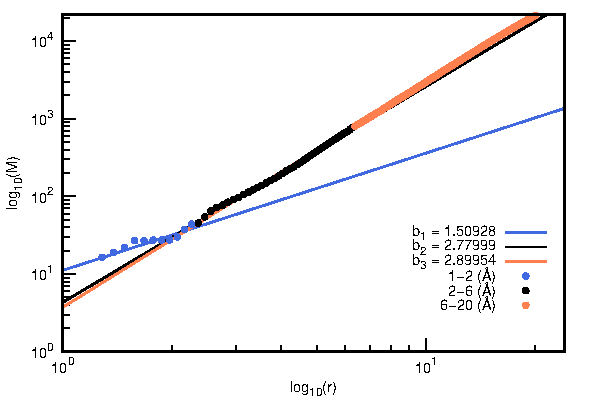
\includegraphics[width=\linewidth,page=1]{graphs/PDBs/1auk/1aukEm.pdf}
				\caption{(2)}
			\end{subfigure}
			
			\vspace{0cm} % Espacio entre filas
			
			\hspace{-0.3cm} 
			\begin{subfigure}{0.49\textwidth}
				\centering
				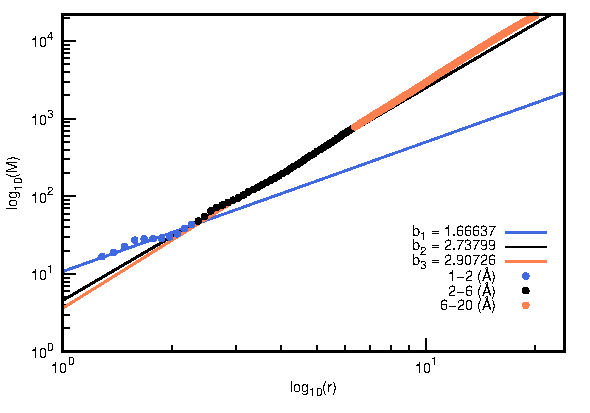
\includegraphics[width=\linewidth,page=1]{graphs/PDBs/1auk/1aukEq.pdf}
				\caption{(3)}
			\end{subfigure}
			\hspace{0.2cm}
			\begin{subfigure}{0.49\textwidth} % M\'{a}s ancho para centrar
				\centering
				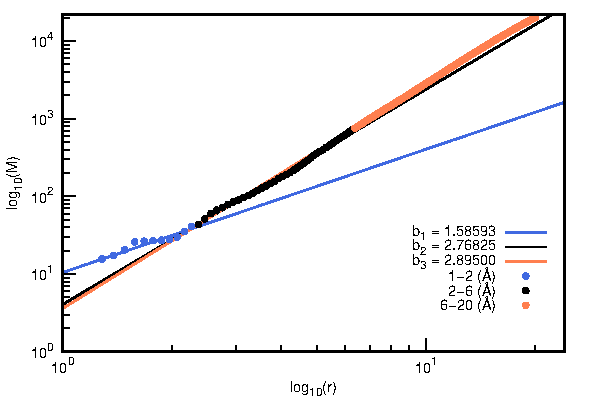
\includegraphics[width=\linewidth,page=1]{graphs/PDBs/1auk/1auk1ns.pdf}
				\caption{(4)}
			\end{subfigure}
			\caption{Regresiones lineales de $log_{10}r$ vs $log_{10}M(r)$ correspondiente a cuatro etapas de procesamiento de la sexta prote\'{i}na con \textit{IdPDB:1auk} de la Tabla \ref{Tabla:ids}: (1) Adici\'{o}n de \'{a}tomos de hidr\'{o}geno al sistema proteico; (2) al minimizar la energ\'{i´}a de la estructura molecular; (3) equilibrando el sistema bajo condiciones termodin\'{a}micas controladas; y (4) despu\'{e}s de una din\'{a}mica molecular de 1 ns.}
			\label{fig:1auk}
		\end{figure}
		
		\begin{figure}[H]
			\subsection*{IdPDB:1b3e}
			
			\hspace{-0.3cm} 
			\begin{subfigure}{0.49\textwidth}
				\centering
				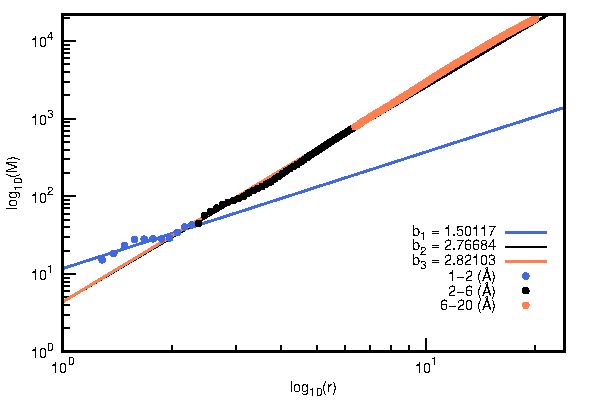
\includegraphics[width=\linewidth,page=1]{graphs/PDBs/1b3e/1b3eaddH.pdf}
				\caption{(1)}
			\end{subfigure}
			\hspace{0.2cm}
			\begin{subfigure}{0.49\textwidth}
				\centering
				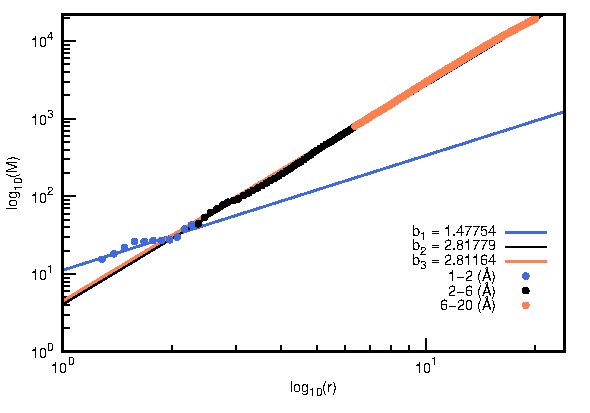
\includegraphics[width=\linewidth,page=1]{graphs/PDBs/1b3e/1b3eEm.pdf}
				\caption{(2)}
			\end{subfigure}
			
			\vspace{0cm} % Espacio entre filas
			
			\hspace{-0.3cm} 
			\begin{subfigure}{0.49\textwidth}
				\centering
				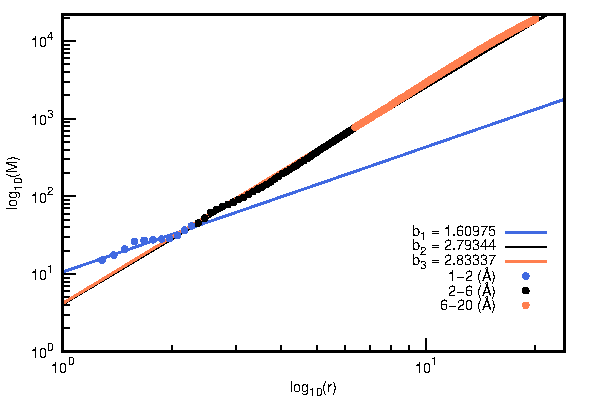
\includegraphics[width=\linewidth,page=1]{graphs/PDBs/1b3e/1b3eEq.pdf}
				\caption{(3)}
			\end{subfigure}
			\hspace{0.2cm}
			\begin{subfigure}{0.49\textwidth} % M\'{a}s ancho para centrar
				\centering
				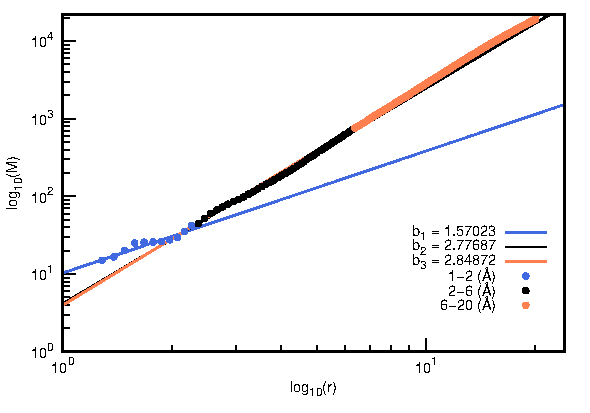
\includegraphics[width=\linewidth,page=1]{graphs/PDBs/1b3e/1b3e1ns.pdf}
				\caption{(4)}
			\end{subfigure}
			\caption{Regresiones lineales de $log_{10}r$ vs $log_{10}M(r)$ correspondiente a cuatro etapas de procesamiento de la s\'{e}ptima prote\'{i}na con \textit{IdPDB:1b3e} de la Tabla \ref{Tabla:ids}: (1) Adici\'{o}n de \'{a}tomos de hidr\'{o}geno al sistema proteico; (2) al minimizar la energ\'{i´}a de la estructura molecular; (3) equilibrando el sistema bajo condiciones termodin\'{a}micas controladas; y (4) despu\'{e}s de una din\'{a}mica molecular de 1 ns.}
			\label{fig:1b3e}
		\end{figure}
		
		
		\begin{figure}[H]
			\subsection*{IdPDB:7khw}
			
			\hspace{-0.3cm} 
			\begin{subfigure}{0.49\textwidth}
				\centering
				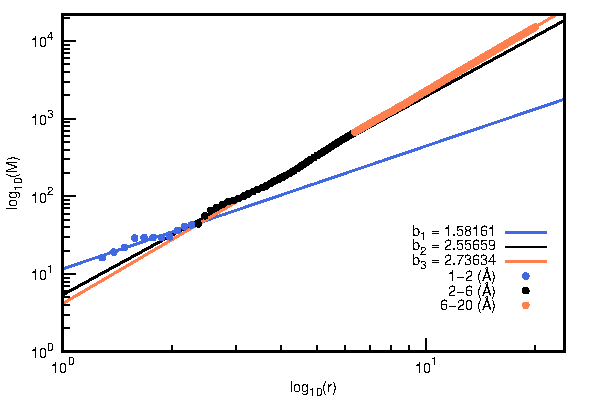
\includegraphics[width=\linewidth,page=1]{graphs/PDBs/7khw/7khwaddH.pdf}
				\caption{(1)}
			\end{subfigure}
			\hspace{0.2cm}
			\begin{subfigure}{0.49\textwidth}
				\centering
				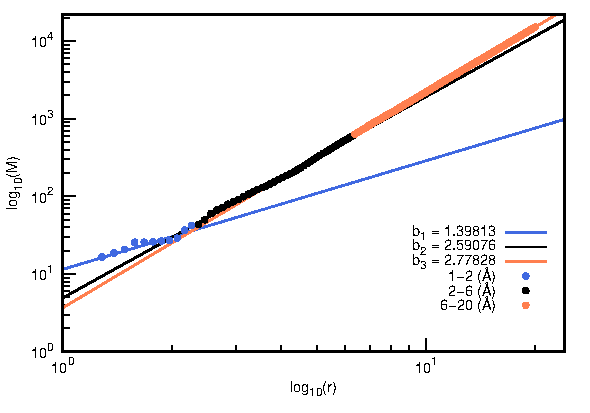
\includegraphics[width=\linewidth,page=1]{graphs/PDBs/7khw/7khwEm.pdf}
				\caption{(2)}
			\end{subfigure}
			
			\vspace{0cm} % Espacio entre filas
			
			\hspace{-0.3cm} 
			\begin{subfigure}{0.49\textwidth}
				\centering
				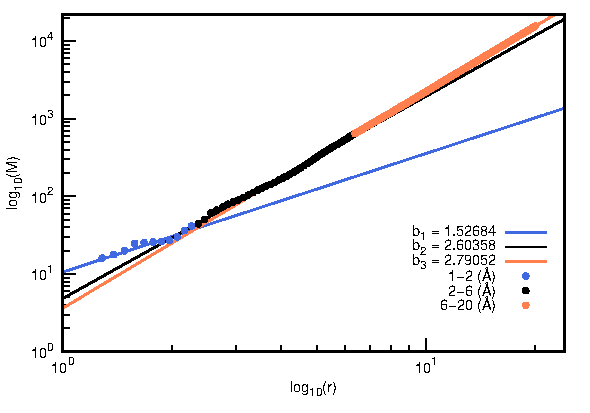
\includegraphics[width=\linewidth,page=1]{graphs/PDBs/7khw/7khwEq.pdf}
				\caption{(3)}
			\end{subfigure}
			\hspace{0.2cm}
			\begin{subfigure}{0.49\textwidth} % M\'{a}s ancho para centrar
				\centering
				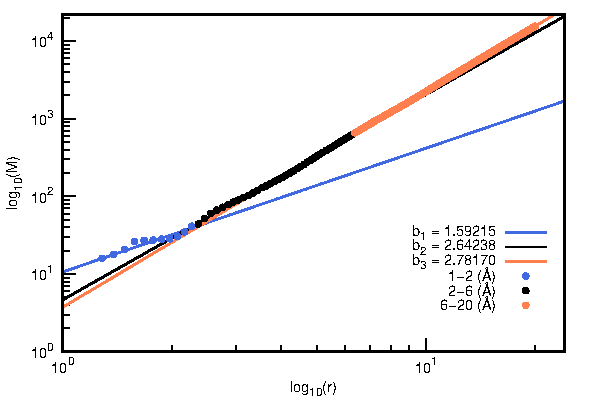
\includegraphics[width=\linewidth,page=1]{graphs/PDBs/7khw/7khw1ns.pdf}
				\caption{(4)}
			\end{subfigure}
			\caption{Regresiones lineales de $log_{10}r$ vs $log_{10}M(r)$ correspondiente a cuatro etapas de procesamiento de la novena prote\'{i}na con \textit{IdPDB:7khw} de la Tabla \ref{Tabla:ids}: (1) Adici\'{o}n de \'{a}tomos de hidr\'{o}geno al sistema proteico; (2) al minimizar la energ\'{i´}a de la estructura molecular; (3) equilibrando el sistema bajo condiciones termodin\'{a}micas controladas; y (4) despu\'{e}s de una din\'{a}mica molecular de 1 ns.}
			\label{fig:7khw}
		\end{figure}
		
		\begin{figure}[H]
			\subsection*{IdPDB:11gs}
			
			\hspace{-0.3cm} 
			\begin{subfigure}{0.49\textwidth}
				\centering
				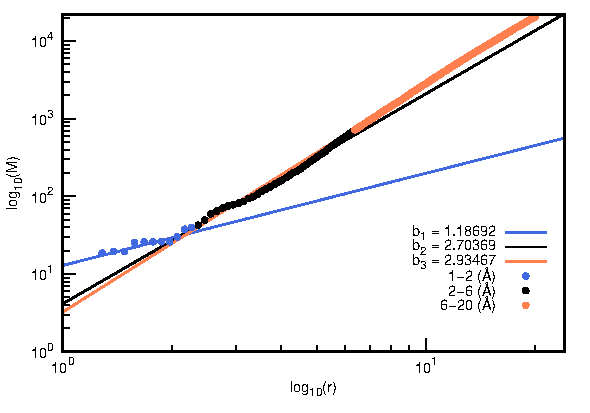
\includegraphics[width=\linewidth,page=1]{graphs/PDBs/11gs/11gsaddH.pdf}
				\caption{(1)}
			\end{subfigure}
			\hspace{0.2cm}
			\begin{subfigure}{0.49\textwidth}
				\centering
				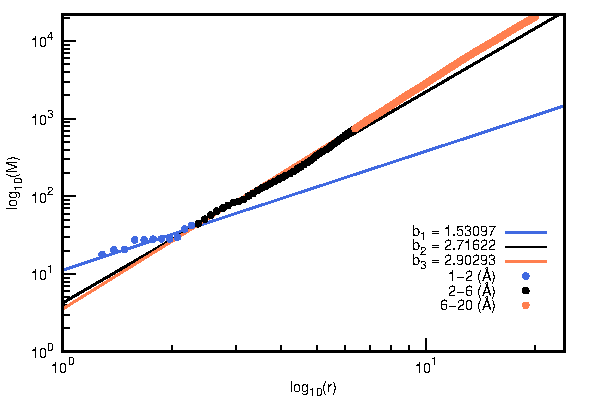
\includegraphics[width=\linewidth,page=1]{graphs/PDBs/11gs/11gsEm.pdf}
				\caption{(2)}
			\end{subfigure}
			
			\vspace{0cm} % Espacio entre filas
			
			\hspace{-0.3cm} 
			\begin{subfigure}{0.49\textwidth}
				\centering
				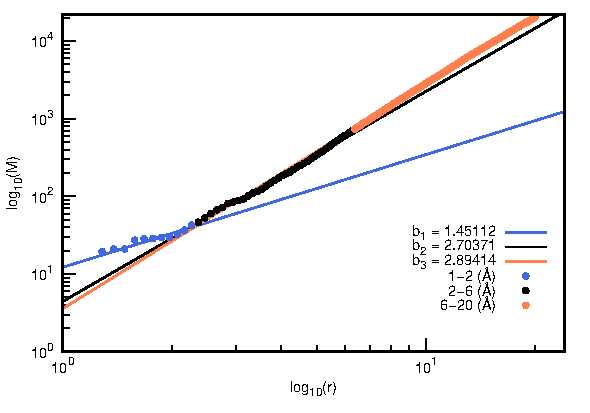
\includegraphics[width=\linewidth,page=1]{graphs/PDBs/11gs/11gsEq.pdf}
				\caption{(3)}
			\end{subfigure}
			\hspace{0.2cm}
			\begin{subfigure}{0.49\textwidth} % M\'{a}s ancho para centrar
				\centering
				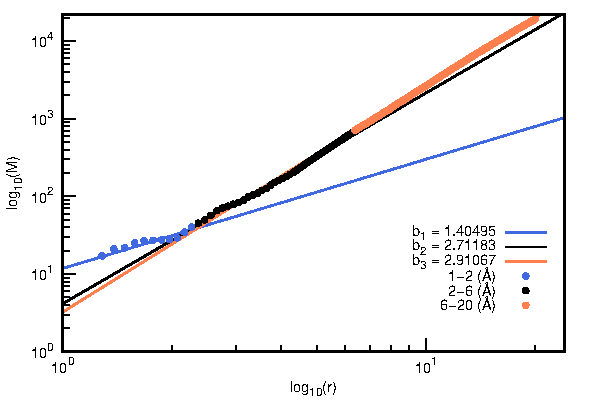
\includegraphics[width=\linewidth,page=1]{graphs/PDBs/11gs/11gs1ns.pdf}
				\caption{(4)}
			\end{subfigure}
			
			\caption{Regresiones lineales de $log_{10}r$ vs $log_{10}M(r)$ correspondiente a cuatro etapas de procesamiento de la octava prote\'{i}na con \textit{IdPDB:11gs} de la Tabla \ref{Tabla:ids}: (1) Adici\'{o}n de \'{a}tomos de hidr\'{o}geno al sistema proteico; (2) al minimizar la energ\'{i´}a de la estructura molecular; (3) equilibrando el sistema bajo condiciones termodin\'{a}micas controladas; y (4) despu\'{e}s de una din\'{a}mica molecular de 1 ns.}
			\label{fig:11gs}
		\end{figure}
		